\documentclass[12pt, letter]{scrartcl}

\setkomafont{section}{%
\Large
}
\setkomafont{subsection}{%
\large
}
\setkomafont{subsubsection}{%
\normalsize
}
\usepackage{multicol}
\usepackage{float}
\usepackage{graphicx}
\usepackage{longtable}
\usepackage{subcaption}
\usepackage{booktabs}
\usepackage{multirow}
\usepackage[T1]{fontenc}
\usepackage[utf8]{inputenc}
\usepackage{lmodern}
\usepackage[margin=1in]{geometry}
\usepackage{setspace}
\usepackage{stackengine}
\PassOptionsToPackage{hyphens}{url}\usepackage{hyperref}
\normalsize
\setlength{\parindent}{4ex}
\setlength{\columnsep}{0.6cm}
\usepackage{titlesec}
\usepackage{enumitem}
\usepackage{tikz}
\tikzstyle{startstop} = [rectangle, rounded corners, minimum width=2cm, minimum height=1.7cm,text centered, draw=black, fill=white]
\tikzstyle{arrow} = [thick,->,>=stealth]
\tikzstyle{arrow2} = [dashed,->,>=stealth]

\newenvironment{figurehere}
  {\def\@captype{figure}}
  {}
  
  \newenvironment{tablehere}
  {\def\@captype{table}}
  {}

\usepackage[english]{babel}
\usepackage{csquotes}

\usepackage[authordate,backend=biber]{biblatex-chicago}
\addbibresource{/Users/andrewmccormack/Desktop/POLI 680/Paper/Tex Proposal 2/political.bib}

\setcounter{topnumber}{2}
\setcounter{bottomnumber}{2}
\setcounter{totalnumber}{4}
\renewcommand{\topfraction}{0.85}
\renewcommand{\bottomfraction}{0.85}
\renewcommand{\textfraction}{0.15}
\renewcommand{\floatpagefraction}{0.7}

\title{{\Large The impact of economic inequality at the local level:} \\ {\Large Preferences for redistributions and perceptions of fairness in England and Wales}}
\date{February 25, 2018}
\author{Andrew McCormack}


\begin{document}


\maketitle
\doublespacing
\section{Introduction}

For the past thirty-five years, income inequality has increased in almost all advanced industrial democracies \parencite{piketty2014, OECD2015together, hopkin2016winner}. In theory, as the majority of citizens in a democratic polity see their share of nation’s wealth decrease relative to those at the top, increasing inequality should lead to a greater political demand for government redistribution \parencite{meltzer1981rational}. Yet, as a variety of political economists have noted, this intuitive expectation does not hold—countries with higher levels of income inequality are systematically less generous than those with a more egalitarian distribution of income \parencite{kenworthy2007inequality, kenworthy2005rising, iversen2009distribution, alesina2004fighting, moene2001inequality}. While a number of historical institutional, political, and cultural explanations have been advanced to explain this phenomenon, I will focus on the role played by democratic citizens’ beliefs about the fairness of the economy as well as their redistributive policy preferences. One prominent strand of literature in the American case argues that, rising inequality concentrates not just economic resources in the hands of top earners, but also political influence \parencite{gilens2012affluence, bartels2008unequal, hacker2010winner}. Along these lines  \textcite[5]{bartels2008unequal} notes that ``[t]he opinions of millions of ordinary citizens in the bottom third of the income distribution have no discernible impact on the behaviour of elected representatives.” By contrast, some have taken issue with the assumptions of this literature that (1) low-income individuals hold consistent opinions on income inequality and (2) that these preferences differ substantially from those of the rich \parencite{soroka2008limits, kelly2010inequality}. This leads to an important empirical question: under what conditions will consistent and coherent attitudes toward inequality and redistribution among low-income earners take hold? Insofar as these conditions can be found, will they drive low-income earners to adopt more cynical perspectives on inequality and more favourable positions toward redistribution?  While a large body of literature explores the determinant of attitudes toward inequality and redistribution at the individual and cross-national level, research in political science has paid little attention to the role played by local context. Utilizing both individual level survey data and local level demographic data, I will contribute to this debate by examining the impact of variation of income inequality at local level. My central expectation is that when individuals directly encounter economic inequality in their day-to-day lives, it will either inaugurate or bring to the fore latent opinions on the fairness of the economy and preferences toward redistribution. 



\section{Background and theoretical expectations}
\vspace{-10pt}
\singlespacing
\subsection{Democratic representation and inequality}
\doublespacing
Political equality is a fundamental premise of democratic government \parencite{dahl1971polyarchy}. Few would disagree that equal representation and equal voice in government decision-making is an ideal by which the performance of democratic government can be judged. To what extent, however, can this ideal be met in the face of rising economic inequality? This question has spurred a large body of literature that documents the limits of representation in unequal societies. \textcite{gilens2012affluence}, for example, finds that the responsiveness of the American political system is strongly biased toward the preferences of the rich, whereas the link between ``what citizens want and what government does'' for the vast majority of Americans is remarkably weak. Similarly, \textcite{bartels2008unequal} claims that politicians are ``utterly unresponsive to the policy preferences of millions of low-income citizens'' and that this unequal representation serves to maintain and reproduce economic inequality. Both Bartels and Gilens reach the conclusion that income inequality is not an inevitable outgrowth of liberal capitalism. For example, Gilens notes that ``policies with clearly downwardly redistributive consequences, such as increases in the minimum wage, are considerably more likely to be adopted under Democratic rule, while policies with upwardly redistributive consequences, such as reductions in the estate tax, are more common when Republicans are in control.'' Likewise, Bartels finds that, despite consistent support among the public for increasing the minimum wage, action has been forestalled by ``conservative Republicans intent of protecting the free market (and low-wage employers) from the predations of people earning \$5.15 per hour.” While the political causes and implications of increasing concentrations of wealth has received the most attention in the American context, income inequality is by no means a uniquely American phenomenon. This raises a broader question: why are advanced industrial democracies, premised on political equality, not producing more egalitarian economic outcomes? The notion that political equality will, or should, lead to the self-correction of economic inequality is premised on the expectation that citizens disadvantaged by the unequal distribution of wealth in their society will recognize this and elect leaders that push for more redistribution. For this reason, the conditions under which individuals form their views about inequality and redistribution are relevant for the broader question.

\subsection{The median voter theorem}

Because rising inequality increases the number of low-income earners relative to high-income earners, we might expect democratic government to keep inequality in check. In this vein, the Meltzer-Richard (MR) model of democracy predict that the median voter has increasingly more to gain from higher taxes and more redistribution under rising inequality and will, in turn, elect office-seeking politicians that have an incentive to implement these policies (Meltzer and Richard 1981). Most scholars agree, albeit frequently not for the same reasons, that this has not been the typical response to rising inequality in advanced industrial democracies \parencite{kenworthy2005rising, iversen2009distribution, bradley2003distribution}. Consequently, “[h]istory reveals a `Robin Hood paradox,' in which redistribution from rich to poor is least present when and where it seems most needed” \parencite{lindert2004growing}. As \textcite[36]{kenworthy2007inequality} note, the premises of the MR model are theoretically questionable. For example, it requires that individuals are aware of the true level of inequality, that the median-income holder will favour greater redistribution when the mean income exceeds their own income, that they will express these preferences via voting, and that the government will respond with more generous redistributive programs. An enormous literature exists on these assumptions, far beyond the scope of this paper. With this in mind, I will focus on the role of attitudes toward inequality and redistribution, as they are an important precondition for how democratic systems will address---or fail to address---rising economic inequality. 

\vspace{15pt}
\singlespacing
\subsection{Are voters aware of the income distribution? Are their preferences toward redistribution really that different from the rich?}
\doublespacing
A great deal of empirical evidence suggests that citizens are relatively uninformed about public affairs, which casts doubt on the notion that most citizens will consider the distribution of wealth, or substantive policy domains more generally, when forming their political attitudes \parencite{kuklinski2000reconsidering, achen2017democracy, converse2006nature}. For instance, Bartels (2008, 146) notes that, citizens' perceptions of economic inequality bear little resemblance to actual trends over time and that the majority of survey respondents have not given much thought to the issue. This reveals an inherent tension in accounts that claim that the preferences of low-income citizens are being ignored as a result of increasing inequality---voters must have these preferences for them to be ignored. More generally, the ``minimalist’’ paradigm of public opinion research claims that the political stands of ordinary citizens ``are, in sum, minimally grounded on political principle, minimally informed by a knowledge of political affairs, minimally stable, and above all, minimally coherent'' \parencite[67]{sniderman2000taking}. If this rather sceptical view of the public holds, the reluctance of democracies to address inequality may stem less from the unresponsiveness on the government than has been claimed, and more from the lack of solid preferences on the part of citizens.

Especially relevant for attitudes toward redistribution, scholars of public opinion have also found that self-interest plays a limited role in predicting political attitudes \parencite{kinder1998opinion, sears1991role}. In this vein, \textcite{soroka2008limits} find a lack of difference in public opinion across income levels in many policy domains. Yet, they do not dispute that policymakers are most responsive to the rich and note that ``with more information and/or mobilization, `real' underlying differences in interests across income levels could ultimately become apparent in policy preferences'' (325). I believe that the local context can provide some guidance in this debate, as the experience of inequality at the local level may provide the means for realizing these differences in interests and, more fundamentally, give low income citizens better understanding of how resources are distributed in their society. Bartels (2008, 6) notes, ``[m]ost Americans have only a vague sense of the contours of the nation’s income distribution---especially for parts of the income distribution that extend beyond their personal experience.'' However, the local level is not beyond the experience of the average citizen. That said, I will discuss in more depth why inequality experienced in the local context might affect attitudes toward inequality and redistribution in the following section.

\vspace{15pt}
\singlespacing
\subsection{The local context}
\doublespacing

Few works exist on the impact of local income inequality on beliefs about the fairness of the economy and redistributive preferences. I believe that economic inequality will exert more of an impact when it is experienced directly. Thus, studying inequality at the local level provides critical leverage---the salience of inequality as a determinant of attitudes toward inequality and redistribution may increase as individuals encounter disparities in wealth throughout their day-to-day lives. \textcite{bartle2017local} find a similar process at play with respect to political participation in the UK---citizens appear more likely to vote where their immediate environment is more economically divided, whereas economic segregation has a depressive effect on turnout. In this vein, the authors suggest ``that when individuals live with others who are relatively similar in socio-economic terms, they will have limited experience of of inequality in the places that they traverse in their daily routines'' (42). If individuals living in relatively economically homogeneous contexts ``are aware of inequality it will be through the media or through a general sense within their community that the area is disadvantaged in comparison to other areas'' (ibid.). On the other hand, when inequality is experience more immediately, it is likely to play a greater role in the formation of attitudes and preferences. The reason for this is that income inequality in the local context may be a more effective source of information about the distribution of wealth in one's society than income inequality in the national context, which is inherently more abstract and less accessible to the average citizen. As \textcite[250]{mondak2000persuasion} note, ``[t]he neighbourhood is of potential political significance simply due to the ready availability of socially transmitted information---information that may complement or counter economic perceptions premised solely on personal or national conditions.'' Indeed, ``[w]hen we look out the front window or walk around the corner, we are exposed to information about the neighborhood, and that information ultimately may contribute to our political judgement'' (ibid.). While the level of aggregation that I consider is larger than the neighbourhood, I expect a similar process to be at play.

 
At this point, it is necessary to draw a distinction between attitudes toward inequality and redistributive preferences. As critics of the MR model have noted, preferences for redistribution are shaped not only by the expected gains and losses from redistribution based on one's current location on the income distribution, but also about by prospects for upward mobility \parencite{benabou2001social}, perceptions of risk \parencite{rehm2009risks}, and beliefs about what determined one's position on the social ladder \parencite{alesina2009preferences, newman2015false}. For instance, individuals may have negative experiences that make them more risk averse and less optimistic about upward mobility, and thus more supportive of social insurance \parencite{alesina2009preferences, margalit2013explaining}. Similarly, \textcite{rehm2009risks} notes that, in addition to income, ``risk exposure'', or uncertainty about future income, also fuels redistributional demand. That is, ``individuals not only demand redistribution because they are poor but also because they are exposed to risks in the labour market'' (872). With respect to beliefs about the determinants of economic success, \textcite{corneo2002individual}, in a cross-national analysis of both Western and formerly socialist countries, find evidence that the belief that income is determined by factors beyond the individual's control may legitimate government policies aimed at reducing inequality. With the exception of \textcite{newman2015false} and \textcite{sands2017exposure}, however, few works exist on how these putative determinants of redistributive preferences as well as preferences for redistribution \textit{as such} are shaped by locally experienced economic inequality. Consequently, I posit that that local inequality may generate or prime feelings about the way wealth is distributed in society. Yet, building on literature from public opinion, it is not immediately clear that this may not affect support for redistribution. 

\subsubsection{Attitudes toward inequality}

I expect that economic inequality at the local level will act as a situational trigger that either galvanizes some underlying predisposition about the unequal distribution of resources in society or informs and mobilizes low-income individuals without such prior predispositions \parencite{sniderman2004predisposing}. When individuals live and work in neighbourhoods that are similar in socio-economic composition, inequality  may not be noticeable in their daily routines.  For instance, \textcite{newman2015false} argue that exposure to high inequality `activates'  a sense of disillusionment among low-income Americans with regard to their beliefs in meritocracy. They find that ``the corrective mechanism theorized by redistributive democracy, at least with respect to a core feature of American ideology [meritocracy], does appear to function, but under a more nuanced set of personal and environmental conditions than identified by scholars in the past.'' A similar process may also be at play with respect to risk exposure. That is, when individuals find themselves at risk of unemployment or some other economic hardship, they may regard it as unjust when they see the security and wealth of others in their daily surroundings. Simply put, when inequality is experienced first-hand, low-income and high-risk individuals will be more aware that others are wealthier than them, and this may strike them as unfair, leading to a shift in attitudes about the fairness of the economy more generally.

At the same time, another branch of the literature on economic inequality argues that the opposite effect holds. Works based on system justification theory (SJT) claim that inequality may \textit{increase} perceptions of the legitimacy of income differences through a psychological motivation to legitimate one's social system \parencite{trump2017income}. For instance, \textcite{solt2016economic, solt2017economic} replicate \textcite{newman2015false} and find that, contrary to authors' claims, lower income people are actually more likely to reject the idea that ``if one works hard, one can get ahead'' in contexts of higher inequality. Similarly, in a series of laboratory and survey experiments, \textcite[20]{trump2017income} finds that ``fixing this knowledge gap [of the true extent of income inequality] would not necessarily raise Americans’ concern with inequality; on the contrary, it may have the counter-intuitive effect of making Americans think of higher income differences as legitimate.'' In short, it is possible that, because humans are predisposed to think of their social system as fair, they internalize the effects of inequality and adjust their expectations to fit the status quo \parencite{jost2004decade}. Thus, it is possible that individuals will be inclined to rationalize economic inequality when it confronts them first-hand. 

One last consideration, agnostic to the direction of the effect of local level inequality, involves the mechanism through which perceptions of the fairness of the economy are formed and expressed. Scholars of public opinion have argued that when individuals are asked to offer an opinion on an issue---especially in the context of a public opinion survey---they will not bring to bear all considerations that are relevant to the issue. Instead, respondents will sample from the considerations that are “at the top of their heads”; the considerations that are the most readily available in memory (Zaller 1992). I expect that when inequality is experienced in an individual's day-to-day life, it will be more readily available a consideration than for those who encounter inequality primarily through the media or conversation. 

With these considerations in mind, the following hypotheses may be formed:

\vspace{15pt}
\singlespacing
\begin{enumerate}[label= \textbf{Hypothesis 1a (H1a)},  leftmargin=*]
  \item \textit{In local contexts where inequality is more pronounced, lower-income individuals will be \textit{more} likely to perceive the economy as unfair, relative to low-income individuals in more equal contexts.}
\end{enumerate}

\begin{enumerate}[label= \textbf{Hypothesis 1b (H1b)},  leftmargin=*]
  \item \textit{In local contexts where inequality is more pronounced, individuals who perceive their livelihoods at risk will be \textit{more} likely to perceive the economy as unfair, relative to at-risk individuals in more equal contexts.}
\end{enumerate}
\doublespacing

On the other hand, if locally-experienced income inequality provokes system justification, we would expect the following:

\vspace{15pt}
\singlespacing
\begin{enumerate}[label= \textbf{Hypothesis 1b (H1b)},  leftmargin=*]
  \item \textit{In local contexts where inequality is more pronounced, lower-income individuals will be \textit{less} likely to perceive the economy as unfair, relative to more equal contexts.}
\end{enumerate}

\doublespacing


\subsubsection{Preferences toward redistribution}

As mentioned above, it is not entirely clear that, even if ``activated'', attitudes about the fairness of the economy will translate into either increased or decreased support for redistribution. Indeed, a great deal of literature on economic voting suggests that when it comes to the determinants of vote choice, considerations about one's own personal financial situation are usually significantly less substantial than how one feels about the economy as a whole \parencite{lewis2013vp}. As \parencite[523]{kinder1979economic} claim, ``[p]rivate economic experience is important, but not for politics. Economic discontents and political judgements inhabit separate domains." At the same time, there is reason to expect that local economic experience may play a role. \textcite[254]{mondak2000persuasion} cite a number of studies on the formation of economic judgements indicating that ``personal experience serves as a default source of political information, to be relied upon only in the absence of more abstract, national-level information.'' In my analysis, I expect a similar process to be at play. That is, when income inequality is pronounced in the local context, low income citizens will use this information to form opinions about broader national-level level policies---that is, redistribution. 

In what direction might we expect local-level inequality to impact redistributive preferences? Based on the preceding section, if low-income and at-risk individuals respond to local income inequality with heightened perceptions of the unfairness of the economy, this may lead to greater support for distribution. Simply put, seeing their neighbours opulence first hand while they struggle to get by and are uncertain about their own future livelihoods, low-income individuals may think: something is wrong with the way wealth is distributed in this country, and something ought to be done about it, which will lead to increased support for redistribution. Alternatively, if local-level income inequality leads to system justification, support for redistribution might decrease among low-income individuals in unequal contexts. For example, low-income earners may justify the income inequality they are confronted with, their affluent neighbours reinforcing the belief that people can get ahead if they work hard. 

\vspace{15pt}
\singlespacing
\begin{enumerate}[label= \textbf{Hypothesis 2a (H2a)},  leftmargin=*]
  \item \textit{In local contexts where inequality is more pronounced, lower-income individuals will be more supportive of government redistribution, relative to more equal contexts.}
\end{enumerate}

\begin{enumerate}[label= \textbf{Hypothesis 2b (H2b)},  leftmargin=*]
  \item \textit{In local contexts where inequality is more pronounced, lower-income individuals will be more supportive of government redistribution, relative to more equal contexts.}
\end{enumerate}

\doublespacing

Alternatively, if SJT holds, we would expect the following:

\vspace{15pt}
\singlespacing
\begin{enumerate}[label= \textbf{Hypothesis 2c (H2c)},  leftmargin=*]
  \item \textit{In local contexts where inequality is more pronounced, lower-income individuals will be less supportive of government redistribution.}
\end{enumerate}
\doublespacing

Before proceeding, it warrants mention that the impact of LA-level inequality may influence preference toward redistribution not through perceptions of fairness but merely through self-interest. Thus, it is entirely possible that local inequality has no impact on perceptions of fairness, but nonetheless stimulates greater support for redistribution because it heightens low-income individuals' awareness of their location on the income distribution. This might, in turn, be informative as to the relative gain they can expect from government redistribution. This is even more likely with respect to perceptions of risk. In fact, while risk exposure may affect perceptions of fairness in unequal contexts, there is not to my knowledge any \textit{a priori} reason to expect that it will provoke system justification. 

\vspace{15pt}
\singlespacing
\section{Data and methods}
\doublespacing

Although my analysis is centered on the influence of local-level income inequality, I  control for a number of individual and local-level factors that may also shape perceptions of fairness and redistributive preferences. For this reason, I draw on data from variety of sources.

\subsection{Local level data}

As the unit of analysis for the local level, I use the local authority (LA) district. Generally speaking, LA districts set the boundaries for a variety of local government arrangements and are a frequently used level of aggregation for a variety of official statistics. As of the 2011 census, the average population per LA district is 161,138, with a standard deviation of 109066.\footnote{The interquartile population range is 93888 to 199823. There are some heavily populated outliers that I may need to take into account to make sure that this is an equivalent measure. See the appendix for a boxplot that illustrates the dispersion of LA populations.} Using available data, I construct two measures of inequality at the local level, detailed below.

There are significant challenges associated with measuring both the level of and distribution of income at local level in the UK, as the UK Census does not collect data on either household or individual incomes. To bridge this gap, the Office for National Statistics (ONS) has produced experimental estimates of average household income for Middle Layer Super Output Areas (MSOAs) \parencite{bond2010understanding}.\footnote{The ONS uses a model-based approach in which estimates are produced by determining a relationship between income measured in the Family Resources Survey (a large scale survey carried out by the ONS) and administrative data for the MSOAs (from the census. The administrative data are used to estimate household income for each MSOA: ``Both sources of data borrow strength from each other to arrive at an unbiased and consistent set of small area estimates that could not be produced from either source in isolation'' \parencite[81]{bond2010understanding}.} Estimates for income inequality at the LA level are constructed using these weekly income estimates from these data. In total, there were 7,201 MSOAs across England and Wales for 2013--2014. The population size of MSOAs range from 5000-15000, with an average population of 7200. Most importantly, there is an average of 21 MSOAs in each LA. Thus, to get a sense of the income distribution in each of the LAs, I take the upper quartile of MSOA weekly income weekly income as a proportion of the lower quartile for each local authority. The advantage of this approach is that it provides an assessment of disparities in wealth between communities in the local authority areas. Where wealthy and poor communities are located within close proximity of one another, income inequality may be a more relevant consideration. In addition, the interpretation is relatively straightforward---as the the upper quartile of MSOAs in a LA become larger relative to the lower quartile, the ratio will take on a greater number, indicating a greater level of inequality.

\begin{figure}[t]
\centering
\vspace{10pt}
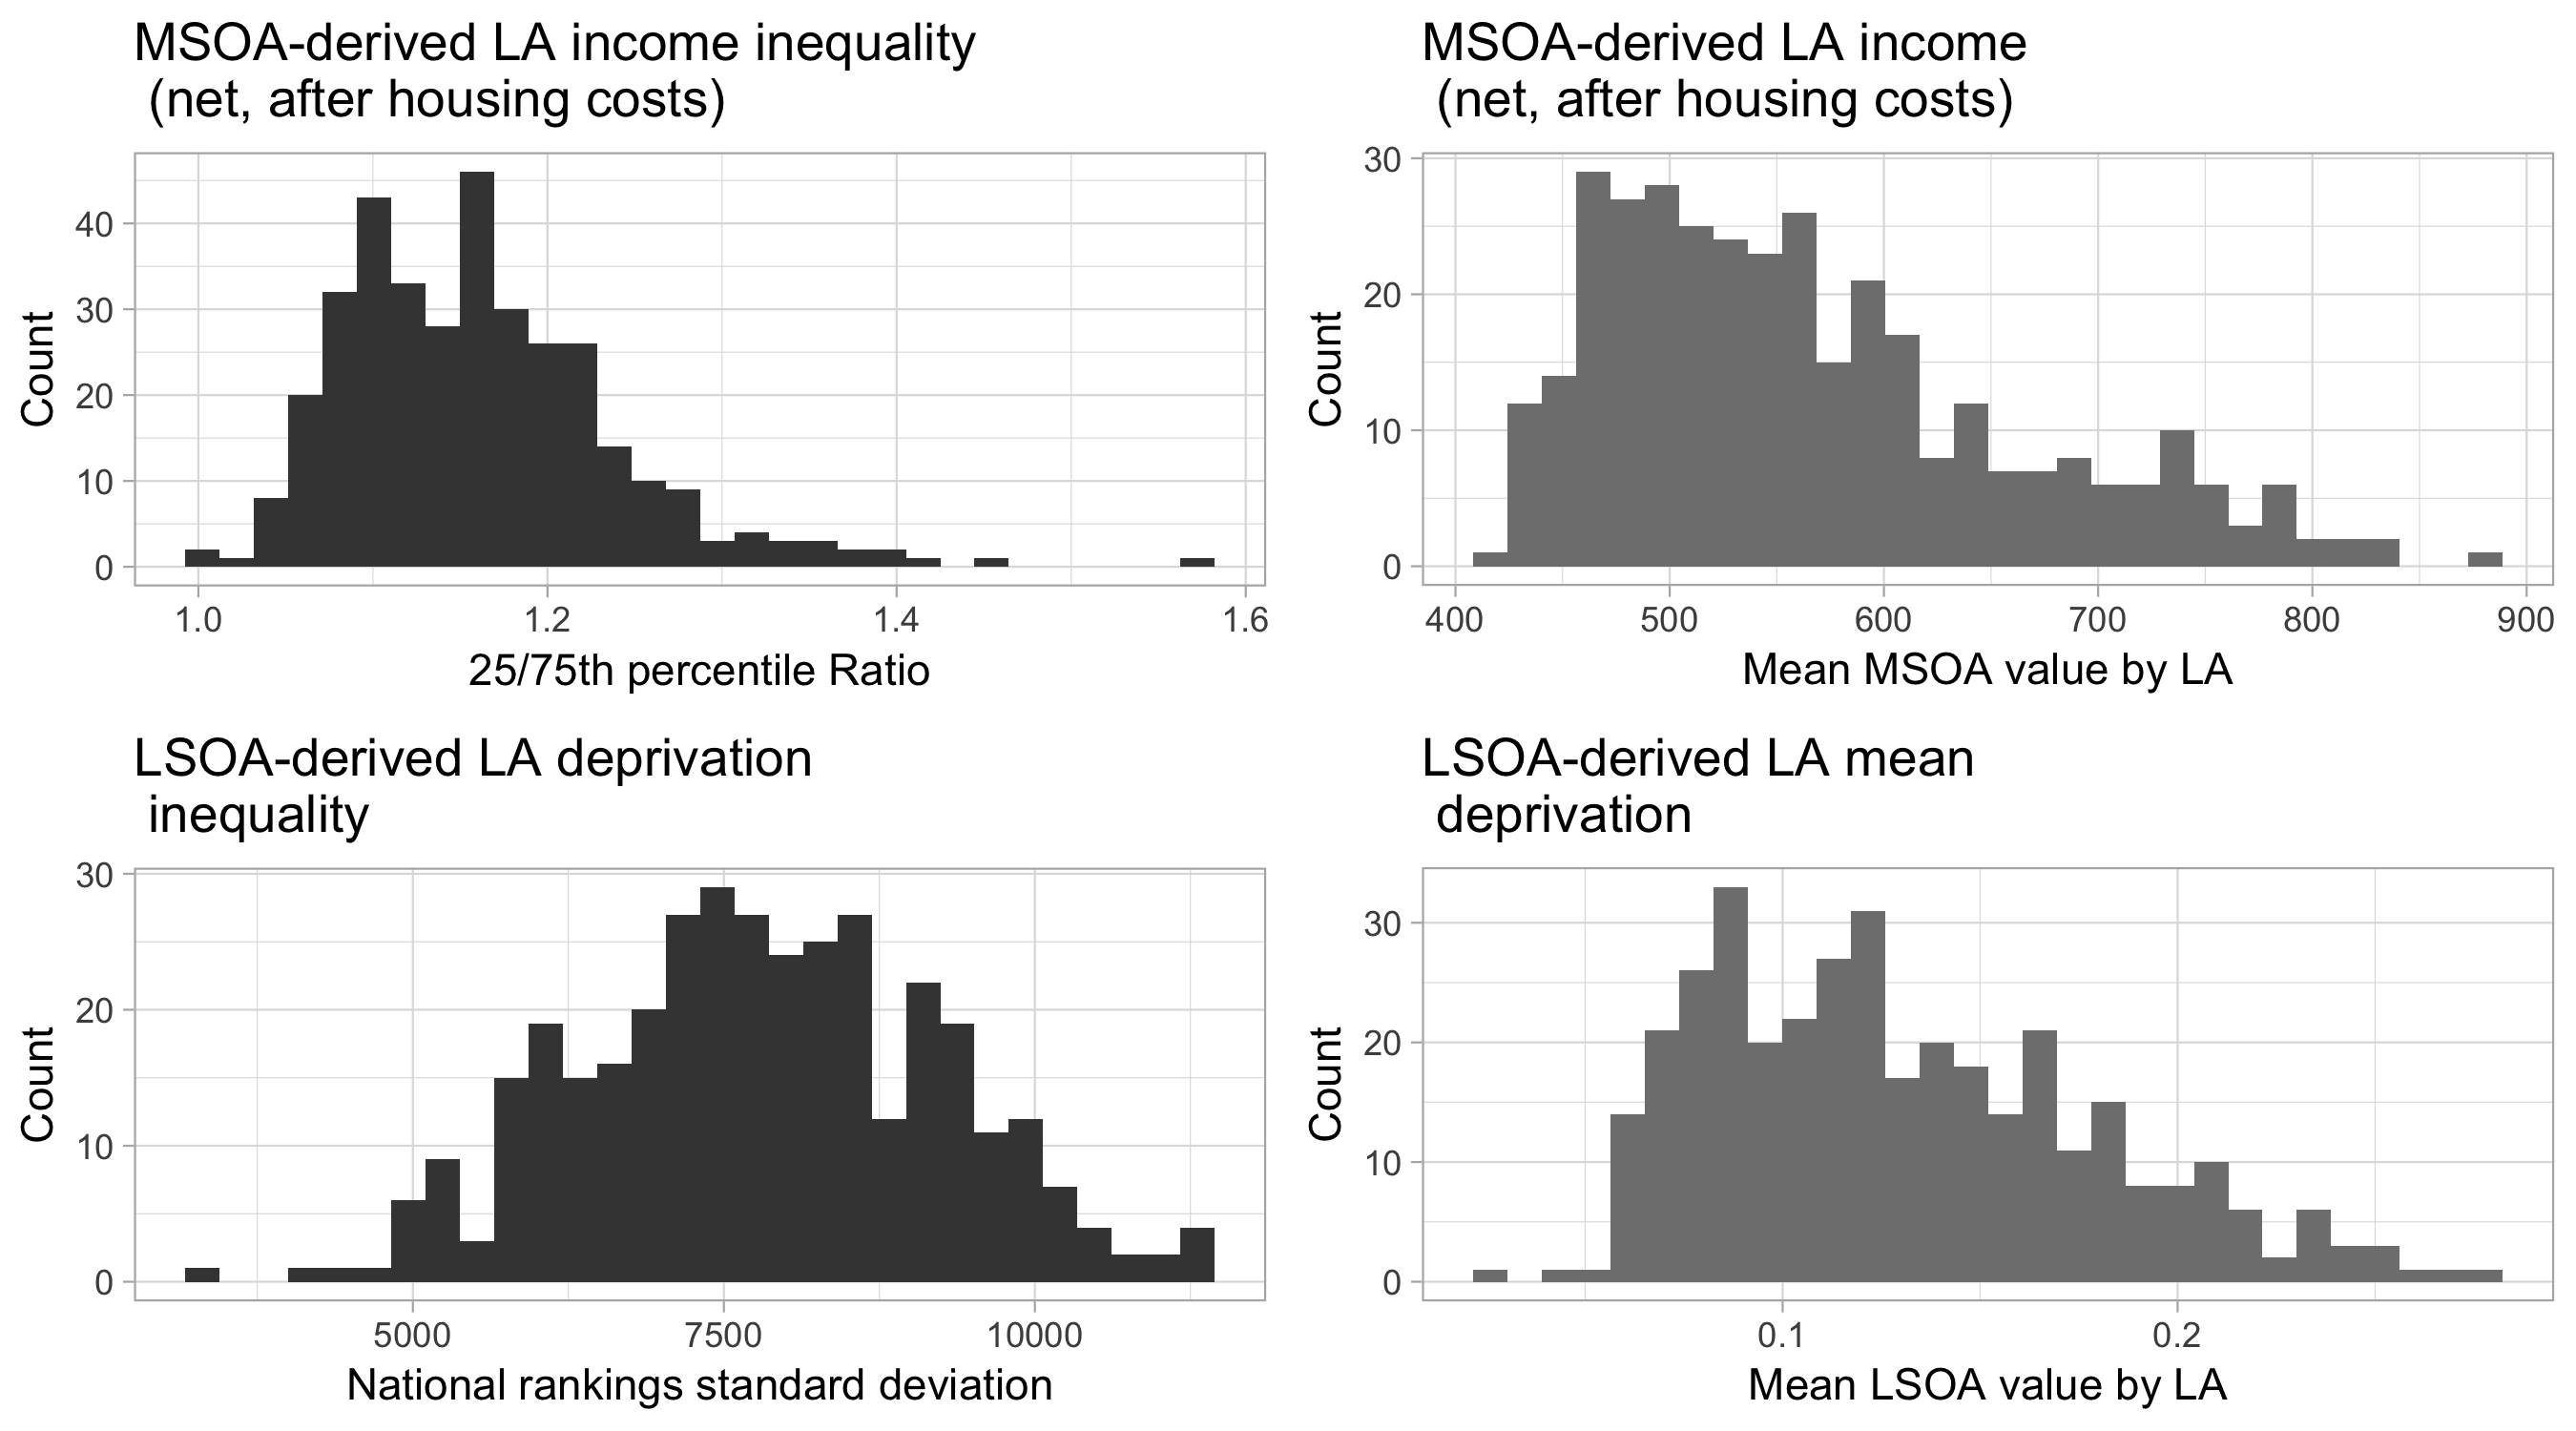
\includegraphics[scale=0.15]{poli680_lainequality.png}
\caption{Distributions of local authority income inequality and mean income measures}
\label{fig:distributions}
\end{figure}

To construct a second measure of local income inequality, I use data on income deprivation from the English Indices of Deprivation 2015 \parencite{deprivation2015} at the Lower Super Output Area (LSOA). There are 32,844 LSOAs in England, with an average population of 1,500. Each LA has an average of 91 LSOAs, with a standard deviation 63. I follow the approach of \textcite{bradshaw2015which} by (1) ranking each LSOA for all of England, (2) grouping the LSOAs within LAs, and (3) taking the standard deviation of the ranks for each LA. Local authorities that have a mix of the most deprived and least deprived LSOAs in terms of income deprivation---i.e. a high standard deviation in terms of deprivation rankings---can be considered less equal than those that have similarly ranked LSOAs. While the interpretation of this measure is less intuitive than, the lower level of aggregation of LSOAs makes it is a more fine-grained and perhaps more accurate measure.

The distributions of MSOA and LSOA inequality are visualized on the left-hand side of ~\ref{fig:distributions}. In my analysis, I also control for the mean values of MSOA income and LSOA deprivation per local authority to ensure that the result is not simply being driven by absolute levels of income. The distribution of these values can be found on the right-hand side of \ref{fig:distributions}. In addition to inequality and mean values of income and deprivation, I also control for LA population density as well at the percentage of individuals in the local authority that are white, as a proxy for ethnic heterogeneity.\footnote{Some argue that increasing ethnic heterogeneity can reduce social solidarity and thus drive down support for redistribution \parencite{alesina2004fighting, garand2017immigration}.} 

\subsection{Individual level variables}

Individual level data for this paper came from an internet panel study conducted from 2014-2017 as part of the British Election Study (BES) \parencite{bespanel}. As I am not exploiting over-time variation, I take the mean values of respondents across waves for continuous and ordinal variables and the modal values for categorical variables (party identification and occupation). 

The primary independent variables are income and risk of unemployment. Income is measured using reported values of annual gross household income and separate into three dichotomous variables: low (less than \textsterling 15,000), mid (between \textsterling 15000 and \textsterling 70,000), and high (\textsterling 70,000 and above). Risk of unemployment is measured with a question that asks respondents: ``During the next 12 months, how likely or unlikely is it that you will be out of a job and looking for work'' and has been also been recoded in three dichotomous categories based on the respondents' level of agreement with this statement: low risk (fairly unlikely and very unlikely), neutral risk (neither likely nor unlikely), and high risk (fairly likely and very likely). 

In addition, I include a standard set of demographic and political control variables for education, age, left-right self-placement, attention paid to politics, and gender. For ease of interpretation, these variables are either dichotomous (in the case of education, gender, party identification, and occupation) or scaled from zero to one (in the case of attention paid to politics and left-right self-placement). Education is coded as a dummy variable that takes on the value of 1 if the respondent completed post-secondary education, whereas occupation takes on the value of one for routine or semi-routine occupations, and zero otherwise. Scores closer to zero and scores closer to one on left right self-placement indicate more left-wing and more right-wing respondents, respectively. Lastly, attention to politics takes on a value closer to zero if the respondent reported paying no attention to politics and closer to one if the respondent reports paying a great deal of attention to politics. 

\subsection{Dependent variables}

The most relevant indicator in the BES that taps into perceptions of economic fairness is an item that asked respondent the degree to which they agree with the statement: ``Ordinary working people do not get their fair share of the nation’s wealth.'' While this variable was originally scaled from zero (strongly disagree) to five (strongly agree), I have recoded it to range from zero to one. This variable is labelled "No Fair share" in subsequent models. The most relevant indicator for attitudes toward redistribution is an item in which respondents read the statement ``Some people feel that government should make much greater efforts to make people's incomes more equal. Other people feel that government should be much less concerned about how equal people’s incomes are. Where would you place yourself on this scale?'' Valid answers range from 0 ``Government should be less concerned about equal incomes'' to 10 ``Government should try to make incomes equal.'' Again, this variable has been recoded from zero to one and is labelled "Redistribution" in subsequent models. In short, higher values on both No fair share and Redistribution indicate higher perceptions of \textit{unfairness} and a greater desire for redistribution, respectively. 


\subsection{Methods}

To test the hypotheses discussed above, I estimate a number of OLS regressions where the key independent variables at the individual level are risk and income and the key independent variable at the LA-level is inequality. Because the data are nested---that is, individual respondents are nested within local authorities---standard errors are clustered at the LA-level. To explain, there are multiple observation per LA (i.e. respondents residing in that LA), which means that these observations will most likely not be independent, violating the assumption that the variables are independent and identically distributed. Ignoring the clustered nature of the data will lead to exaggerated levels of statistical significance on coefficient estimates \parencite{moulton1990illustration}. Cluster-adjusted standard errors allow observations within a cluster to be correlated, but requires the assumption that observations across clusters are independent \parencite{primo2007estimating}. While multilevel modelling is another suitable method for modeling nested data, I have opted for the clustered standard errors approach as this method requires fewer assumptions of the data and provides for greater ease of interpretation \parencite{steenbergen2002modeling}. 

Because I expect the impact of income on perceptions of fairness and redistributive preferences to be partially conditional on local-level inequality, I include in each model a cross-level interaction between (1) income or risk and (2) local-level inequality. Whether or not local-level income inequality has a discernible impact is dependent on these key parameters. 

\begin{table}[t]
\caption{The impact of MSOA income inequality}
\centering
\setlength{\tabcolsep}{0.4em}
\scalebox{0.74}{
\begin{tabular}{l c c c c c c c c}
\toprule[1.5pt]
& \multicolumn{8}{c}{\textit{Dependent variable:}} \\[5pt]
& \multicolumn{2}{c}{No fair share} & \multicolumn{2}{c}{Redistribution} & \multicolumn{2}{c}{No fair share} & \multicolumn{2}{c}{Redistribution} \\
\textbf{Individual-level variables} & (1) & (2) & (3) & (4) & (5) & (6) & (7) & (8) \\ 
\cmidrule[1pt](lr){2-3} \cmidrule[1pt](lr){4-5} \cmidrule[1pt](lr){6-7} \cmidrule[1pt](lr){8-9}

High income                                 & $-0.08^{***}$ & $-0.09^{***}$ & $-0.08^{***}$ & $-0.10^{***}$ &               &               &               &               \\
                                            & $(0.01)$      & $(0.02)$      & $(0.00)$      & $(0.01)$      &               &               &               &               \\
Low income                                  & $0.02^{***}$  & $0.02^{**}$   & $0.06^{***}$  & $0.06^{***}$  &               &               &               &               \\
                                            & $(0.00)$      & $(0.01)$      & $(0.00)$      & $(0.01)$      &               &               &               &               \\
High risk                                   &               &               &               &               & $0.05^{***}$  & $0.02^{*}$    & $0.04^{***}$  & $0.03^{*}$    \\
                                            &               &               &               &               & $(0.00)$      & $(0.01)$      & $(0.00)$      & $(0.01)$      \\
Low risk                                    &               &               &               &               & $-0.03^{***}$ & $-0.04^{***}$ & $-0.04^{***}$ & $-0.05^{***}$ \\
                                            &               &               &               &               & $(0.00)$      & $(0.01)$      & $(0.00)$      & $(0.01)$      \\
\multicolumn{9}{l}{\textbf{Local authority-level variables}} \\[5pt]
MSOA inequality                             & $0.00$        & $0.01$        & $0.00$        & $0.00$        & $0.01$        & $-0.00$       & $0.00$        & $-0.01$       \\
                                            & $(0.01)$      & $(0.01)$      & $(0.01)$      & $(0.01)$      & $(0.01)$      & $(0.01)$      & $(0.01)$      & $(0.01)$      \\
MSOA mean                                   & $-0.04^{***}$ & $-0.04^{***}$ & $-0.03^{***}$ & $-0.03^{***}$ & $-0.06^{***}$ & $-0.07^{***}$ & $-0.05^{***}$ & $-0.05^{***}$ \\
                                            & $(0.01)$      & $(0.01)$      & $(0.01)$      & $(0.01)$      & $(0.01)$      & $(0.01)$      & $(0.01)$      & $(0.01)$      \\
\multicolumn{5}{l}{\textbf{Interactions}} \\[5pt]
High income $\times$ MSOA inequality        &               & $0.06^{*}$    &               & $0.02$        &               &               &               &               \\
                                            &               & $(0.03)$      &               & $(0.02)$      &               &               &               &               \\
Low income $\times$ MSOA inequality         &               & $-0.04^{**}$  &               & $-0.01$       &               &               &               &               \\
                                            &               & $(0.02)$      &               & $(0.02)$      &               &               &               &               \\
High income $\times$ MSOA mean              &               & $-0.01$       &               & $0.02$        &               &               &               &               \\
                                            &               & $(0.03)$      &               & $(0.02)$      &               &               &               &               \\
Low income $\times$ MSOA mean               &               & $0.03$        &               & $0.01$        &               &               &               &               \\
                                            &               & $(0.02)$      &               & $(0.02)$      &               &               &               &               \\
High risk $\times$ MSOA inequality          &               &               &               &               &               & $0.02$        &               & $0.04$        \\
                                            &               &               &               &               &               & $(0.02)$      &               & $(0.03)$      \\
Low risk $\times$ MSOA inequality           &               &               &               &               &               & $0.02$        &               & $0.01$        \\
                                            &               &               &               &               &               & $(0.01)$      &               & $(0.02)$      \\
High risk $\times$ MSOA mean                &               &               &               &               &               & $0.06^{***}$  &               & $-0.00$       \\
                                            &               &               &               &               &               & $(0.02)$      &               & $(0.02)$      \\
Low risk $\times$ MSOA mean                 &               &               &               &               &               & $0.01$        &               & $0.00$        \\
                                            &               &               &               &               &               & $(0.01)$      &               & $(0.01)$      \\
Intercept                                   & $0.78^{***}$  & $0.78^{***}$  & $0.77^{***}$  & $0.77^{***}$  & $0.79^{***}$  & $0.80^{***}$  & $0.80^{***}$  & $0.89^{***}$  \\
                                            & $(0.02)$      & $(0.02)$      & $(0.02)$      & $(0.03)$      & $(0.04)$      & $(0.04)$      & $(0.02)$      & $(0.05)$      \\
\hline
R$^2$                                       & 0.30          & 0.30          & 0.36          & 0.36          & 0.30          & 0.30          & 0.36          & 0.36          \\
Adj. R$^2$                                  & 0.30          & 0.30          & 0.36          & 0.36          & 0.30          & 0.30          & 0.35          & 0.35          \\
Num. obs.                                   & 28530         & 28530         & 28043         & 28043         & 35365         & 35365         & 34631         & 34631         \\
RMSE                                        & 0.18          & 0.18          & 0.21          & 0.21          & 0.18          & 0.18          & 0.21          & 0.21          \\
\toprule[1.5pt]
\multicolumn{9}{l}{\normalsize{$^{***}p<0.001$, $^{**}p<0.01$, $^*p<0.05$}} \\[-4pt]
\multicolumn{9}{l}{\multirow{3}{590pt}{\normalsize{\textit{Notes:} Individual and local-authority level controls not reported (see Appendix \ref{appendix:msoafull} for full results). Standard errors clustered by local authority. All independent and dependent variables have been scaled to range from 0 to 1.}}} \\
\\
\end{tabular}}
\label{table:msoatable}
\end{table}


\section{Results}

As all of the hypotheses discussed above involve the impact of income and risk on perceptions of fairness and attitudes toward redistribution \textit{conditional on local-level inequality}, it is necessary to plot the marginal effects of income and risk across different levels of inequality. Thus, results are presented in regression tables as well as marginal effects plots. As this analysis is primarily concerned with the impact of local-level inequality, the regression tables (Table~\ref{table:msoatable} and Table~\ref{table:lsoatable}) found below do not report coefficients for individual-level and LA-level controls. Full results can be found in Appendix \ref{appendix:msoafull}.

\subsection{MSOA income inequality}

\begin{figure}[t]
\caption{Marginal effects of income on perceptions of unfairness and preferences for redistribution by local inequality}
\centering
\vspace{10pt}
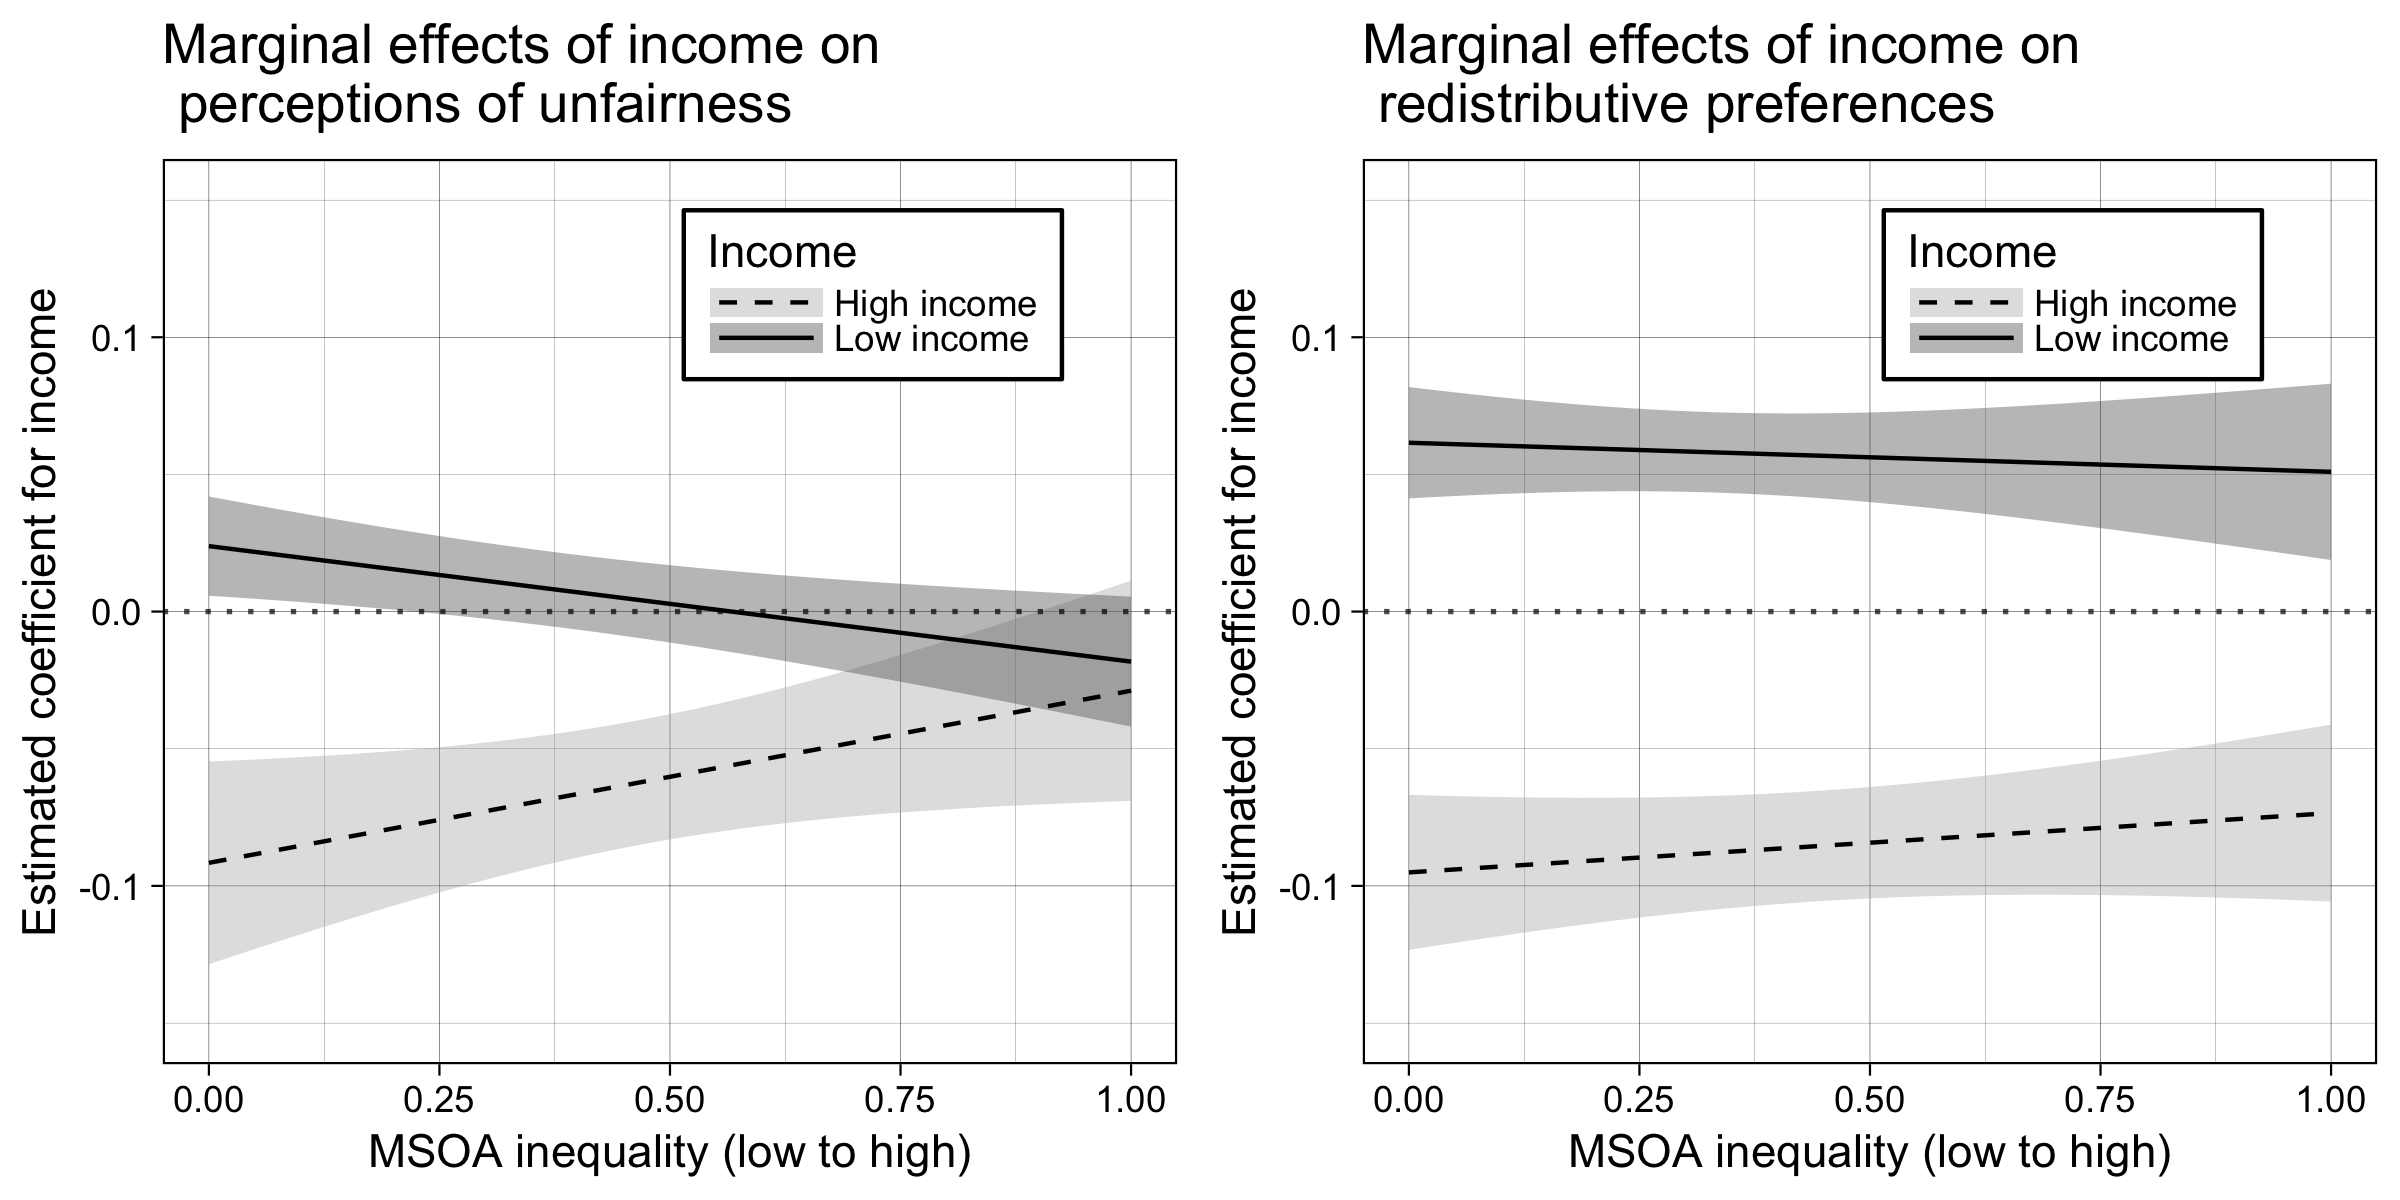
\includegraphics[scale=0.16]{b1to2.png}
\label{fig:12}
{\footnotesize \\ \textit{Note:} The figure shows the interaction effects of income and local inequality from column (2) and (4) of Table~\ref{table:msoatable}. Confidence bands are 95\% confidence intervals. standard errors clustered by local authority. \par}
\end{figure}

\begin{figure}[t]
\caption{Marginal effects of risk on perceptions of unfairness and preferences for redistribution by local inequality}
\centering
\vspace{10pt}
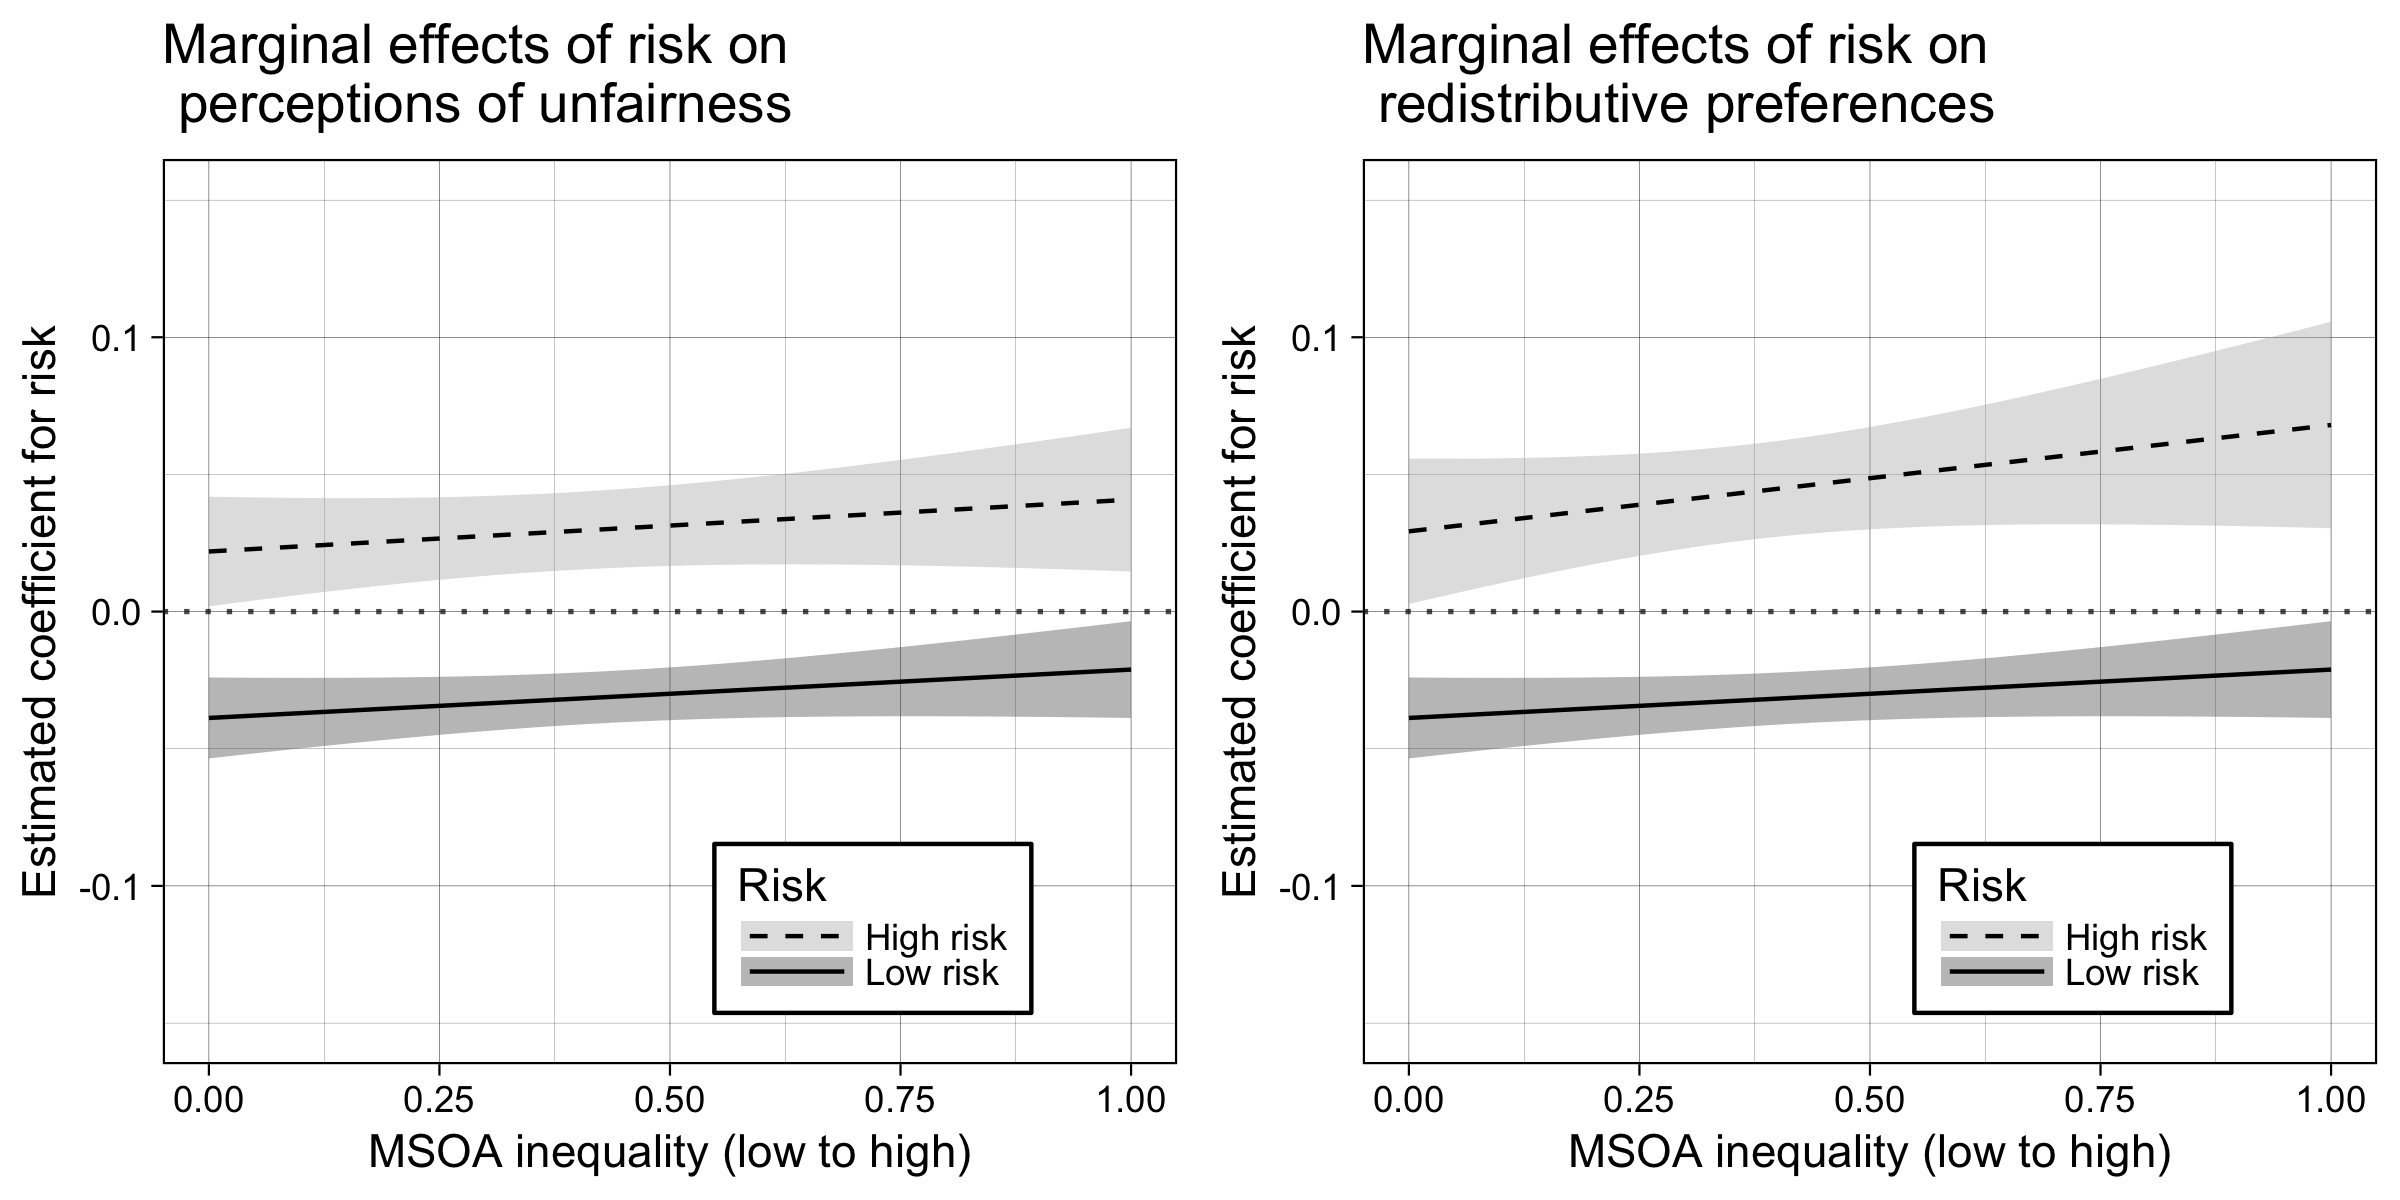
\includegraphics[scale=0.16]{b3to4.png}
\label{fig:34}
{\footnotesize \\ \textit{Note:} The figure shows the interaction effects of risk and local inequality from column (6) and (8) of Table~\ref{table:msoatable}. Confidence bands are 95\% confidence intervals. standard errors clustered by local authority.\par}
\end{figure}

Beginning with models based on MSOA-derived measures of inequality (Table~\ref{table:msoatable}), the interaction between MSOA inequality and either income or risk reaches statistical significance only in model (2), which considers the effect on fairness perceptions associated with low-income earners at different levels of inequality. The coefficient on Low income $\times$ MSOA inequality indicates the impact on perceptions of fairness that low income respondents experience for a one unit increase in inequality, over and above the effect of inequality for respondents who are not low income. In this case, a one unit increase means going from the least (0) to the most (1) unequal context. That said, the coefficient on the Low income $\times$ MSOA inequality indicates a decrease of four points. While statistically significant at the 99 percent level, this decrease is rather modest. Moreover, the marginal effects of this interaction, visualized on the left hand side of Figure~\ref{fig:12}, indicates that the effect associated with low income respondents is only statistically significant at very low levels of inequality. Interestingly, the change associated with high income respondents is positive---that is, when local inequality rises, high income respondents appear slightly more inclined to believe that ordinary citizens do not get their fair share of wealth. Lastly, the relatively straight lines on the right hand side of Figure~\ref{fig:12} echoes what is found in model (4)---while low income respondents are about 6 points more in favour and high income respondents about 10 points less in favour redistribution relative the mid-income group, the effect does not seem to change across different levels of inequality. 

With respect to risk and redistributive attitudes, the slightly positive slopes in Figure~\ref{fig:34}---which pertain to columns (6) and (8) of Table~\ref{table:msoatable}---suggest that, regardless of risk level, rising inequality increases both feelings of unfairness and preferences for redistribution. Nonetheless, because these slopes do not reach statistical significance at conventional levels, they are merely suggestive. 

Although the interaction effects of inequality and either risk or income are mostly null throughout Table~\ref{table:msoatable}, the baseline effects associated with low-income and at-risk respondents, found in columns (1), (3), (5), and (7), suggest that these groups do in fact perceive the economy as more unfair and are more favourable to redistribution relative to other respondents. Yet, while statistically significant, these effect are all less than 10 points, which is a rather modest. If low-income individuals have truly distinct preferences with respect to redistribution, we might expect to see a stronger effect. As to the four hypotheses stated above, while model (2) provides very modest support to H1a---that is, low-income respondents appear slightly less likely to perceive the economy as unfair in unequal context---the remaining hypotheses cannot be confirmed.

\begin{table}[t]
\caption{The impact of LSOA income inequality}
\centering
\setlength{\tabcolsep}{0.4em}
\scalebox{0.74}{
\begin{tabular}{l c c c c c c c c}
\toprule[1.5pt]
& \multicolumn{8}{c}{\textit{Dependent variable:}} \\[5pt]
& \multicolumn{2}{c}{No fair share} & \multicolumn{2}{c}{Redistribution} & \multicolumn{2}{c}{No fair share} & \multicolumn{2}{c}{Redistribution} \\
\textbf{Individual-level variables} & (1) & (2) & (3) & (4) & (5) & (6) & (7) & (8) \\ 
\cmidrule[1pt](lr){2-3} \cmidrule[1pt](lr){4-5} \cmidrule[1pt](lr){6-7} \cmidrule[1pt](lr){8-9}
High income                                 & $-0.08^{***}$ & $-0.11^{***}$ & $-0.08^{***}$ & $-0.09^{***}$ &               &               &               &               \\
                                            & $(0.01)$      & $(0.02)$      & $(0.01)$      & $(0.02)$      &               &               &               &               \\
Low income                                  & $0.02^{***}$  & $0.04^{**}$   & $0.06^{***}$  & $0.06^{***}$  &               &               &               &               \\
                                            & $(0.00)$      & $(0.01)$      & $(0.00)$      & $(0.01)$      &               &               &               &               \\
High risk                                   &               &               &               &               & $0.05^{***}$  & $0.07^{***}$  & $0.04^{***}$  & $0.01^{***}$  \\
                                            &               &               &               &               & $(0.00)$      & $(0.01)$      & $(0.01)$      & $(0.02)$      \\
Low risk                                    &               &               &               &               & $-0.03^{***}$ & $-0.04^{***}$ & $-0.04^{***}$ & $-0.06^{***}$ \\
                                            &               &               &               &               & $(0.00)$      & $(0.01)$      & $(0.00)$      & $(0.01)$      \\
\multicolumn{5}{l}{\textbf{Local authority-level variables}} \\[5pt]
LSOA Inequality                             & $0.00$        & $-0.00$       & $-0.02^{*}$   & $-0.02^{*}$   & $0.01$        & $-0.00$       & $-0.01$       & $-0.03^{*}$   \\
                                            & $(0.01)$      & $(0.01)$      & $(0.01)$      & $(0.01)$      & $(0.01)$      & $(0.01)$      & $(0.01)$      & $(0.01)$      \\
LSOA Mean                                   & $0.04^{***}$  & $0.05^{***}$  & $0.04^{***}$  & $0.04^{***}$  & $0.05^{***}$  & $0.06^{***}$  & $0.06^{***}$  & $0.06^{***}$  \\
                                            & $(0.01)$      & $(0.01)$      & $(0.01)$      & $(0.01)$      & $(0.01)$      & $(0.01)$      & $(0.01)$      & $(0.01)$      \\
\multicolumn{5}{l}{\textbf{Interactions}} \\[5pt]
High income $\times$ LSOA inequality        &               & $0.02$        &               & $0.01$        &               &               &               &               \\
                                            &               & $(0.03)$      &               & $(0.03)$      &               &               &               &               \\
Low income $\times$ LSOA inequality         &               & $0.01$        &               & $0.01$        &               &               &               &               \\
                                            &               & $(0.02)$      &               & $(0.02)$      &               &               &               &               \\
High income $\times$ LSOA mean              &               & $0.07^{**}$   &               & $0.02$        &               &               &               &               \\
                                            &               & $(0.02)$      &               & $(0.02)$      &               &               &               &               \\
Low income $\times$ LSOA mean               &               & $-0.06^{**}$  &               & $-0.02$       &               &               &               &               \\
                                            &               & $(0.02)$      &               & $(0.02)$      &               &               &               &               \\
High risk $\times$ LSOA inequality          &               &               &               &               &               & $0.00$        &               & $0.05$        \\
                                            &               &               &               &               &               & $(0.02)$      &               & $(0.03)$      \\
Low risk $\times$ LSOA inequality           &               &               &               &               &               & $0.02$        &               & $0.03$        \\
                                            &               &               &               &               &               & $(0.01)$      &               & $(0.02)$      \\
High risk $\times$ LSOA mean                &               &               &               &               &               & $-0.05^{**}$  &               & $-0.02$       \\
                                            &               &               &               &               &               & $(0.02)$      &               & $(0.02)$      \\
Low risk $\times$ LSOA mean                 &               &               &               &               &               & $-0.00$       &               & $-0.00$       \\
                                            &               &               &               &               &               & $(0.01)$      &               & $(0.02)$      \\
Intercept                                   & $0.75^{***}$  & $0.74^{***}$  & $0.74^{***}$  & $0.74^{***}$  & $0.74^{***}$  & $0.74^{***}$  & $0.75^{***}$  & $0.76^{***}$  \\
                                            & $(0.02)$      & $(0.02)$      & $(0.02)$      & $(0.02)$      & $(0.02)$      & $(0.02)$      & $(0.02)$      & $(0.02)$      \\
\hline
R$^2$                                       & 0.30          & 0.30          & 0.36          & 0.36          & 0.30          & 0.30          & 0.36          & 0.36          \\
Adj. R$^2$                                  & 0.30          & 0.30          & 0.36          & 0.36          & 0.30          & 0.30          & 0.36          & 0.36          \\
Num. obs.                                   & 25657         & 25657         & 25202         & 25202         & 31824         & 31824         & 31146         & 31146         \\
RMSE                                        & 0.19          & 0.19          & 0.21          & 0.21          & 0.19          & 0.19          & 0.22          & 0.22          \\
\toprule[1.5pt]
\multicolumn{9}{l}{\normalsize{$^{***}p<0.001$, $^{**}p<0.01$, $^*p<0.05$}} \\[-4pt]
\multicolumn{9}{l}{\multirow{3}{590pt}{\normalsize{\textit{Notes:} Individual and local-authority level controls not reported (see Appendix \ref{appendix:lsoafull} for full results). Standard errors clustered by local authority. All independent and dependent variables have been scaled to range from 0 to 1.}}} \\
\\
\end{tabular}}
\label{table:lsoatable}
\end{table}


\subsection{LSOA deprivation inequality}

Using income at the MSOA level to calculate measures of inequality at the LA level may lack precision, resulting in estimates of limited validity. For this reason, I run models with the alternative measure of inequality, constructed with measures of income deprivation at a lower level of aggregation, the LSOA. Unfortunately, running models with this measure of inequality brings us no closer to a significant interaction effect between income or risk and local level inequality. There is no evidence that LSOA inequality generates or primes attitudes toward inequality or redistribution for low income or at risk either respondents in either of the directions hypothesized above. 

Although the results in Table~\ref{table:lsoatable} cannot confirm my hypotheses, the overall effect of income deprivation runs in an intuitive direction---that is, respondents from LAs with higher income deprivation appear to perceive the economy as less fair and are in favour of more distribution. Moreover, the overall impact of LSOA inequality in model 3 appears to have a slightly negative impact on redistributive attitudes ($\beta = -0.02$, $p = 0.031$), though the limited magnitude of this effect makes it difficult to draw a firm conclusion. 

Figures \ref{fig:56} and \ref{fig:78} tell a similar story to that of Figures \ref{fig:12} and \ref{fig:34}: while lower income and at risk respondents appear to be generally more likely to perceive the economy as unfair and more supportive of redistribution than the rich and secure, this relationship does not seem to change across different levels of local inequality. However, much like in \ref{fig:56}, the slightly positive slopes on the right hand side of Figure \ref{fig:78} suggest that, for both high and low risk respondents, increasing local-level inequality may increase support for redistribution. Once again, however, column (8) in Table~\ref{table:lsoatable} indicates that this is not a significant effect. 


\begin{figure}[t]
\caption{Marginal effects of income on perceptions of unfairness and preferences for redistribution by local inequality}
\centering
\vspace{10pt}
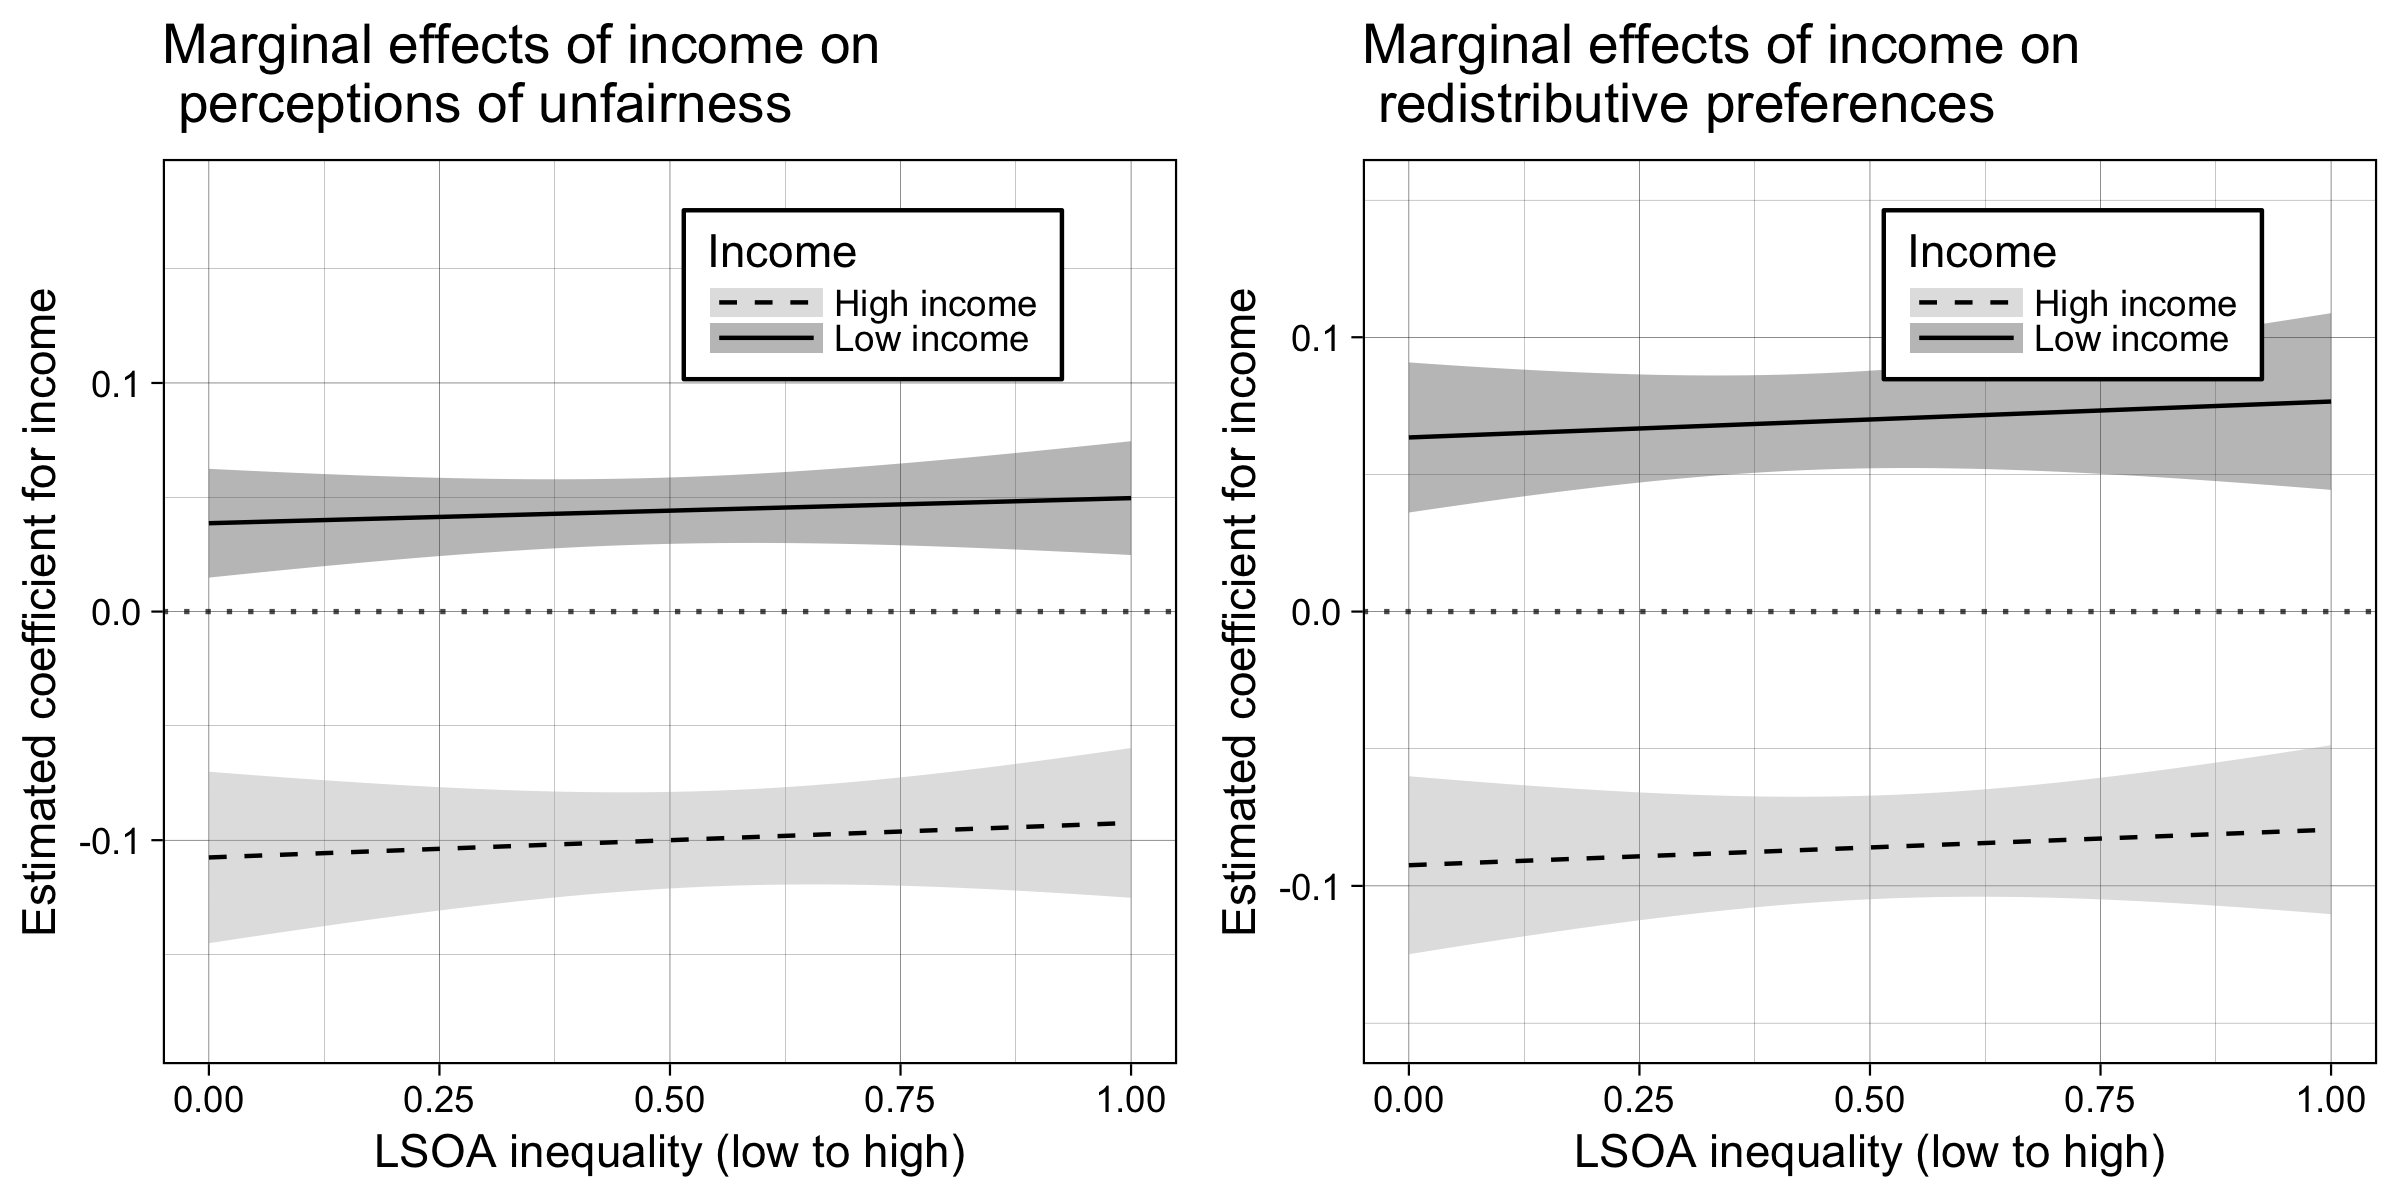
\includegraphics[scale=0.16]{b5to6.png}
\label{fig:56}
{\footnotesize \\ \textit{Note:} The figure shows the interaction effects of income and local inequality from column (2) and (4) of Table~\ref{table:msoatable}. Confidence bands are 95\% confidence intervals. standard errors clustered by local authority. \par}
\end{figure}

\begin{figure}[h]
\caption{Marginal effects of risk on perceptions of unfairness and preferences for redistribution by local inequality}
\centering
\vspace{10pt}
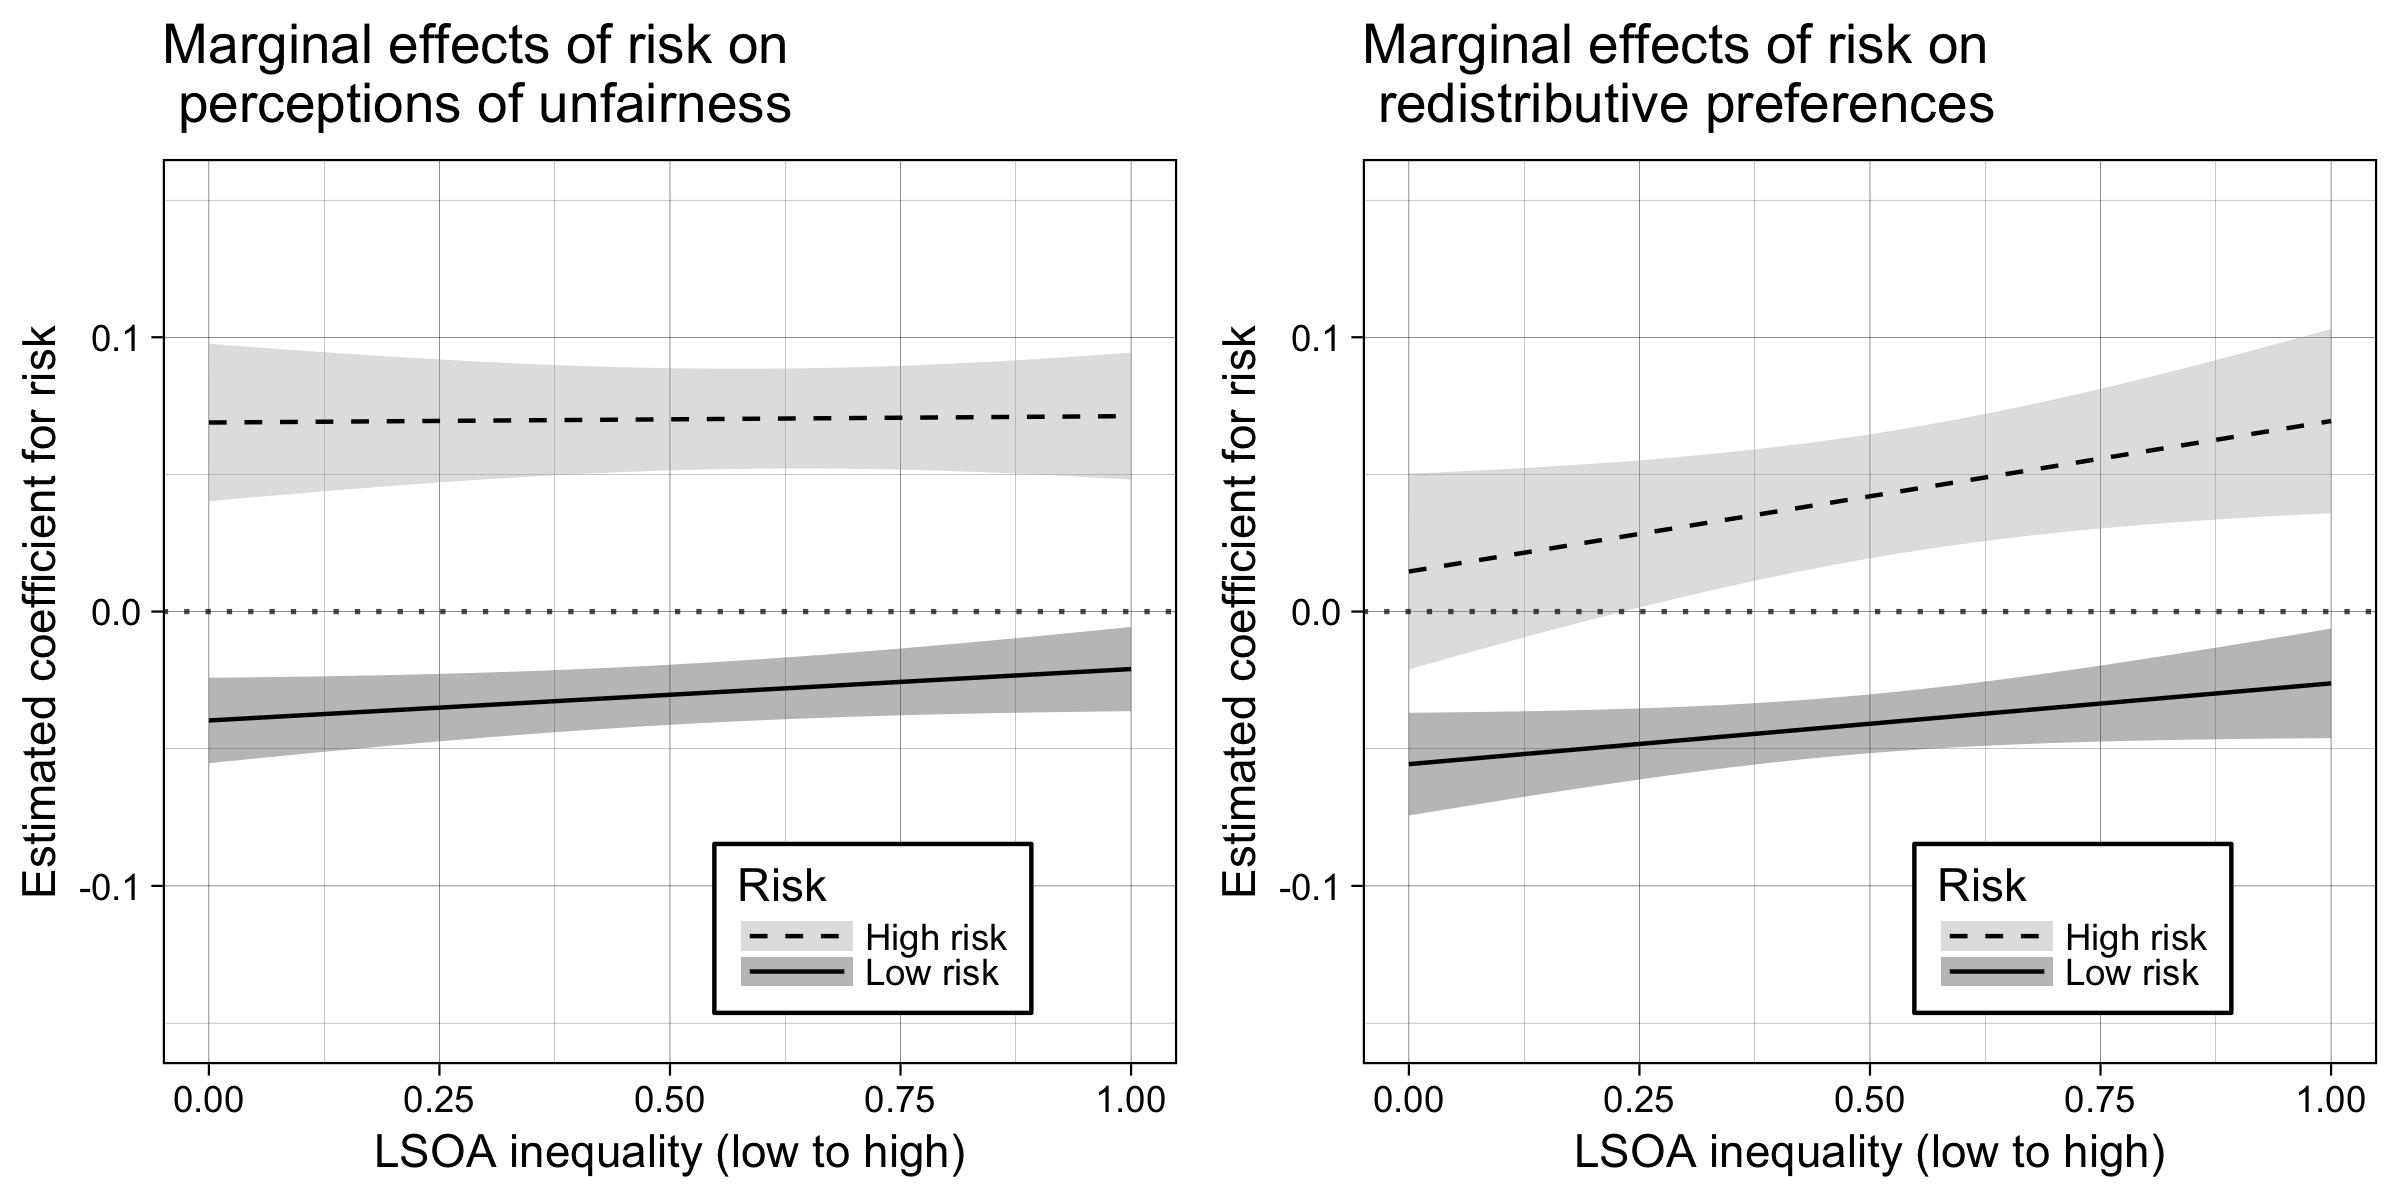
\includegraphics[scale=0.16]{b7to8.png}
\label{fig:78}
{\footnotesize \\ \textit{Note:} The figure shows the interaction effects of risk and local inequality from column (6) and (8) of Table~\ref{table:msoatable}. Confidence bands are 95\% confidence intervals. standard errors clustered by local authority.\par}
\end{figure}

\subsection{Conclusion}

Many observers have noted that, contrary to theoretical expectations of majoritarian models of democracy premised on the economic self-interest of voters, democratic governments have generally not responded to rising income inequality with more redistribution. For some, economic inequality concentrates not only economic resources, but also political power in the hands of the rich, which results in limited political reponsiveness of the putative redistributive preferences of lower income groups \parencite{bartels2008unequal, gilens2012affluence}. Others object to the notion that lower income citizens' hold distinctive views about the income distribution and what should be done about it \parencite{soroka2008limits}. Indeed, a large body of public opinion research claims that individuals' are often ill-informed about public policy and lack the ability to form coherent policy preferences \parencite{kuklinski2000reconsidering, sniderman2000taking, achen2017democracy}. Furthermore, it has been demonstrated that citizens' preferences toward redistribution are not merely a function of their current location on the income distribution \parencite{meltzer1981rational}, but also their prospects for upward mobility \parencite{benabou2001social}, the extent to which they believe inequality is justified \parencite{alesina2009preferences, trump2017income}, and their exposure to and experience of economic risk \parencite{rehm2009risks}. 

With these considerations in mind, this paper sought to determine whether the experience of inequality at the local level stimulates perceptions of the fairness of the economy or preferences toward redistribution. In other words, I hypothesized that while income inequality at the country level does not lead to a rejection of the economic system from those disadvantage by it, this may occur at a lower level of aggregation where inequality is more apparent in individuals' daily lives. Alternative, the possibility was kept open that local level inequality may stimulate system justification and drive down support for redistribution. Despite my theoretical expectations that local-level income inequality would affect lower income and at-risk individuals' perceptions of the fairness of the economy as well as their support of government redistribution, little evidence was found to this end. While the reasons for this are not entirely clear, a number of explanations---both empirical and theoretical---may explain the null results.

Empirically, the local authority level may be too large a level of aggregation to capture the direct experience of inequality.\footnote{The empirical limitations of using LSOA income deprivation and MSOA income estimates to construct measure of inequality is perhaps the most serious empirical problem. This is discussed in relative detail in Section 3 (Results) and thus will not receive much further attention here.} For instance, with an average of 161,138 individuals in each LA, it is entirely possible that low income and at-risk respondents live and work in economically homogeneous enclaves within LAs and are not in fact exposed to inequality in their day-to-day lives, despite living in LAs that are unequal overall. 

Theoretically, it may be that income inequality is not the most relevant local determinant of economic attitudes and policy preferences. For instance, \parencite[403]{rehm2012risk} argues that ``[t]he welfare state has two natural constituencies: the disadvantaged and the insecure'' and that, where disadvantage and insecurity are cross-cutting, there are likely to be broader encompassing coalitions in support of the welfare state. Along these lines, we may expect support for redistribution to be higher in disadvantaged LAs where large amounts of individuals are employed in declining industries.\footnote{While this may drive up support for redistribution in a given LA, the overlap of risk and disadvantage, according to Rehm, will not lead to cross-class coalitions in support of the welfare state.} Another possibility, though less likely, is that some individuals justify the inequality they are confronted with whereas others regard it as unfair. In this case, these two countervailing tendencies would cancel out the overall effect of local-level inequality. 

Although I was unable to find empirical support for the idea that local-level income inequality impacts perceptions of fairness and preferences for redistribution, the role of inequality at the local level merits further research. Indeed, a majority of the literature on economic inequality has focused almost solely on national-level inequality while, as \parencite{glaeser2009inequality} notes ``most people live in cities and their experience of inequality is shaped by their local environment.'' In this vein, the authors find that unequal places have higher murder rates, people say they are less happy, and, after controlling for the skill distribution of the area, have slower population growth. With more robust measurements of local-level inequality and well-constructed survey items, future research can further unravel the political implications of inequality as it is experienced in the democratic citizen's day to day life.

\singlespacing

\section{The impact of MSOA inequality---full models}
\label{appendix:msoafull}


\begin{tiny}
\setlength{\tabcolsep}{0.2em}
\begin{longtable}{lcccccccc}
\caption[The impact of MSOA income inequality]{The impact of MSOA income inequality}\\
& \multicolumn{8}{c}{\textit{Dependent variable:}} \\[5pt]
& \multicolumn{2}{c}{No fair share} & \multicolumn{2}{c}{Redistribution} & \multicolumn{2}{c}{No fair share} & \multicolumn{2}{c}{Redistribution} \\
& (1) & (2) & (3) & (4) & (5) & (6) & (7) & (8) \\ 
\toprule[1pt]
\multicolumn{9}{l}{\textbf{Individual level variables}} \\[5pt]
High income                                 & $-0.08^{***}$ & $-0.09^{***}$ & $-0.08^{***}$ & $-0.10^{***}$ &               &               &               &               \\
                                            & $(0.01)$      & $(0.02)$      & $(0.00)$      & $(0.01)$      &               &               &               &               \\
Low income                                  & $0.02^{***}$  & $0.02^{**}$   & $0.06^{***}$  & $0.06^{***}$  &               &               &               &               \\
                                            & $(0.00)$      & $(0.01)$      & $(0.00)$      & $(0.01)$      &               &               &               &               \\
High risk                                   &               &               &               &               & $0.05^{***}$  & $0.02^{*}$    & $0.04^{***}$  & $0.03^{*}$    \\
                                            &               &               &               &               & $(0.00)$      & $(0.01)$      & $(0.00)$      & $(0.01)$      \\
Low risk                                    &               &               &               &               & $-0.03^{***}$ & $-0.04^{***}$ & $-0.04^{***}$ & $-0.05^{***}$ \\
                                            &               &               &               &               & $(0.00)$      & $(0.01)$      & $(0.00)$      & $(0.01)$      \\
Post-secondary education                    & $-0.02^{***}$ & $-0.02^{***}$ & $-0.03^{***}$ & $-0.03^{***}$ & $-0.03^{***}$ & $-0.03^{***}$ & $-0.04^{***}$ & $-0.04^{***}$ \\
                                            & $(0.00)$      & $(0.00)$      & $(0.00)$      & $(0.00)$      & $(0.00)$      & $(0.00)$      & $(0.00)$      & $(0.00)$      \\
Routine/semi-routine occupation             & $0.03^{***}$  & $0.03^{***}$  & $0.04^{***}$  & $0.04^{***}$  & $0.03^{***}$  & $0.03^{***}$  & $0.04^{***}$  & $0.04^{***}$  \\
                                            & $(0.00)$      & $(0.00)$      & $(0.00)$      & $(0.00)$      & $(0.00)$      & $(0.00)$      & $(0.00)$      & $(0.00)$      \\
Age                                         & $0.01^{***}$  & $0.01^{***}$  & $0.00^{***}$  & $0.00^{***}$  & $0.01^{***}$  & $0.01^{***}$  & $0.00^{**}$   & $0.00^{**}$   \\
                                            & $(0.00)$      & $(0.00)$      & $(0.00)$      & $(0.00)$      & $(0.00)$      & $(0.00)$      & $(0.00)$      & $(0.00)$      \\
Age$^2$                                     & $-0.00^{***}$ & $-0.00^{***}$ & $-0.00^{***}$ & $-0.00^{***}$ & $-0.00^{***}$ & $-0.00^{***}$ & $-0.00$       & $-0.00$       \\
                                            & $(0.00)$      & $(0.00)$      & $(0.00)$      & $(0.00)$      & $(0.00)$      & $(0.00)$      & $(0.00)$      & $(0.00)$      \\
Left-right                                  & $-0.29^{***}$ & $-0.29^{***}$ & $-0.46^{***}$ & $-0.46^{***}$ & $-0.29^{***}$ & $-0.29^{***}$ & $-0.46^{***}$ & $-0.46^{***}$ \\
                                            & $(0.01)$      & $(0.01)$      & $(0.01)$      & $(0.01)$      & $(0.01)$      & $(0.01)$      & $(0.01)$      & $(0.01)$      \\
Attention to politics                       & $0.06^{***}$  & $0.06^{***}$  & $0.02^{**}$   & $0.02^{**}$   & $0.04^{***}$  & $0.04^{***}$  & $0.01$        & $0.01$        \\
                                            & $(0.01)$      & $(0.01)$      & $(0.01)$      & $(0.01)$      & $(0.01)$      & $(0.01)$      & $(0.01)$      & $(0.01)$      \\
Female                                      & $0.00$        & $0.00$        & $0.02^{***}$  & $0.02^{***}$  & $0.00$        & $0.00$        & $0.02^{***}$  & $0.02^{***}$  \\
                                            & $(0.00)$      & $(0.00)$      & $(0.00)$      & $(0.00)$      & $(0.00)$      & $(0.00)$      & $(0.00)$      & $(0.00)$      \\
\multicolumn{9}{l}{\textbf{Local authority-level variables}} \\[5pt]
MSOA inequality                             & $0.00$        & $0.01$        & $0.00$        & $0.00$        & $0.01$        & $-0.00$       & $0.00$        & $-0.01$       \\
                                            & $(0.01)$      & $(0.01)$      & $(0.01)$      & $(0.01)$      & $(0.01)$      & $(0.01)$      & $(0.01)$      & $(0.01)$      \\
MSOA mean                                   & $-0.04^{***}$ & $-0.04^{***}$ & $-0.03^{***}$ & $-0.03^{***}$ & $-0.06^{***}$ & $-0.07^{***}$ & $-0.05^{***}$ & $-0.05^{***}$ \\
                                            & $(0.01)$      & $(0.01)$      & $(0.01)$      & $(0.01)$      & $(0.01)$      & $(0.01)$      & $(0.01)$      & $(0.01)$      \\
Percent white                               & $-0.05^{**}$  & $-0.05^{**}$  & $-0.04^{*}$   & $-0.04^{*}$   & $-0.02$       & $-0.02$       & $-0.01$       & $-0.02$       \\
                                            & $(0.02)$      & $(0.02)$      & $(0.02)$      & $(0.02)$      & $(0.01)$      & $(0.01)$      & $(0.02)$      & $(0.02)$      \\
Population density                          & $-0.00$       & $-0.00$       & $0.00$        & $0.00$        & $-0.00$       & $-0.00$       & $0.00$        & $0.00$        \\
                                            & $(0.00)$      & $(0.00)$      & $(0.00)$      & $(0.00)$      & $(0.00)$      & $(0.00)$      & $(0.00)$      & $(0.00)$      \\
\multicolumn{5}{l}{\textbf{Party identification (baseline party: Labour)}} \\[5pt]
British National Party (BNP)                & $0.03$        & $0.03$        & $0.10^{*}$    & $0.10^{*}$    &               &               & $0.08^{*}$    &               \\
                                            & $(0.04)$      & $(0.04)$      & $(0.05)$      & $(0.05)$      &               &               & $(0.04)$      &               \\
Conservative                                & $-0.14^{***}$ & $-0.14^{***}$ & $-0.13^{***}$ & $-0.13^{***}$ & $-0.15^{***}$ & $-0.15^{***}$ & $-0.14^{***}$ & $-0.22^{***}$ \\
                                            & $(0.00)$      & $(0.00)$      & $(0.01)$      & $(0.01)$      & $(0.04)$      & $(0.04)$      & $(0.01)$      & $(0.04)$      \\
Green Party                                 & $0.01$        & $0.01$        & $0.02^{*}$    & $0.02^{*}$    & $0.01$        & $0.00$        & $0.02^{**}$   & $-0.06$       \\
                                            & $(0.01)$      & $(0.01)$      & $(0.01)$      & $(0.01)$      & $(0.04)$      & $(0.04)$      & $(0.01)$      & $(0.04)$      \\
Liberal Democrat                            & $-0.06^{***}$ & $-0.06^{***}$ & $-0.05^{***}$ & $-0.05^{***}$ & $-0.07$       & $-0.07$       & $-0.05^{***}$ & $-0.13^{**}$  \\
                                            & $(0.00)$      & $(0.00)$      & $(0.01)$      & $(0.01)$      & $(0.04)$      & $(0.04)$      & $(0.00)$      & $(0.04)$      \\
Other/don't know/none                       & $-0.04^{***}$ & $-0.04^{***}$ & $-0.04^{***}$ & $-0.04^{***}$ & $-0.04$       & $-0.04$       & $-0.04^{***}$ & $-0.13^{**}$  \\
                                            & $(0.00)$      & $(0.00)$      & $(0.00)$      & $(0.00)$      & $(0.04)$      & $(0.04)$      & $(0.00)$      & $(0.04)$      \\
Plaid Cymru                                 & $0.02$        & $0.02$        & $-0.00$       & $-0.00$       & $0.00$        & $0.00$        & $-0.00$       & $-0.09$       \\
                                            & $(0.01)$      & $(0.01)$      & $(0.02)$      & $(0.02)$      & $(0.04)$      & $(0.04)$      & $(0.01)$      & $(0.04)$      \\
Scottish National Party (SNP)               & $-0.04$       & $-0.04$       & $-0.03$       & $-0.04$       & $-0.04$       & $-0.04$       & $0.09$        & $0.01$        \\
                                            & $(0.06)$      & $(0.06)$      & $(0.03)$      & $(0.03)$      & $(0.07)$      & $(0.07)$      & $(0.07)$      & $(0.08)$      \\
United Kingdom Independence Party (UKIP)    & $0.01^{*}$    & $0.01^{*}$    & $-0.02^{**}$  & $-0.02^{**}$  & $0.01$        & $0.00$        & $-0.02^{**}$  & $-0.11^{*}$   \\
                                            & $(0.01)$      & $(0.01)$      & $(0.01)$      & $(0.01)$      & $(0.04)$      & $(0.04)$      & $(0.01)$      & $(0.04)$      \\
\multicolumn{5}{l}{\textbf{Interactions}} \\[5pt]
High income $\times$ MSOA inequality        &               & $0.06^{*}$    &               & $0.02$        &               &               &               &               \\
                                            &               & $(0.03)$      &               & $(0.02)$      &               &               &               &               \\
Low income $\times$ MSOA inequality         &               & $-0.04^{**}$  &               & $-0.01$       &               &               &               &               \\
                                            &               & $(0.02)$      &               & $(0.02)$      &               &               &               &               \\
High income $\times$ MSOA mean              &               & $-0.01$       &               & $0.02$        &               &               &               &               \\
                                            &               & $(0.03)$      &               & $(0.02)$      &               &               &               &               \\
Low income $\times$ MSOA mean               &               & $0.03$        &               & $0.01$        &               &               &               &               \\
                                            &               & $(0.02)$      &               & $(0.02)$      &               &               &               &               \\
High risk $\times$ MSOA inequality          &               &               &               &               &               & $0.02$        &               & $0.04$        \\
                                            &               &               &               &               &               & $(0.02)$      &               & $(0.03)$      \\
Low risk $\times$ MSOA inequality           &               &               &               &               &               & $0.02$        &               & $0.01$        \\
                                            &               &               &               &               &               & $(0.01)$      &               & $(0.02)$      \\
High risk $\times$ MSOA mean                &               &               &               &               &               & $0.06^{***}$  &               & $-0.00$       \\
                                            &               &               &               &               &               & $(0.02)$      &               & $(0.02)$      \\
Low risk $\times$ MSOA mean                 &               &               &               &               &               & $0.01$        &               & $0.00$        \\
                                            &               &               &               &               &               & $(0.01)$      &               & $(0.01)$      \\
Intercept                                   & $0.78^{***}$  & $0.78^{***}$  & $0.77^{***}$  & $0.77^{***}$  & $0.79^{***}$  & $0.80^{***}$  & $0.80^{***}$  & $0.89^{***}$  \\
                                            & $(0.02)$      & $(0.02)$      & $(0.02)$      & $(0.03)$      & $(0.04)$      & $(0.04)$      & $(0.02)$      & $(0.05)$      \\
\hline
R$^2$                                       & 0.30          & 0.30          & 0.36          & 0.36          & 0.30          & 0.30          & 0.36          & 0.36          \\
Adj. R$^2$                                  & 0.30          & 0.30          & 0.36          & 0.36          & 0.30          & 0.30          & 0.35          & 0.35          \\
Num. obs.                                   & 28530         & 28530         & 28043         & 28043         & 35365         & 35365         & 34631         & 34631         \\
RMSE                                        & 0.18          & 0.18          & 0.21          & 0.21          & 0.18          & 0.18          & 0.21          & 0.21          \\
\toprule[1.5pt]
\multicolumn{9}{l}{\scriptsize{$^{***}p<0.001$, $^{**}p<0.01$, $^*p<0.05$}}
\end{longtable}
\end{tiny}


\section{The impact of LSOA inequality---full models}
\label{appendix:lsoafull}

\begin{tiny}
\setlength{\tabcolsep}{0.2em}
\begin{longtable}{lcccccccc}
\caption[The impact of LSOA income inequality]{The impact of LSOA income inequality}\\
& \multicolumn{8}{c}{\textit{Dependent variable:}} \\[5pt]
& \multicolumn{2}{c}{No fair share} & \multicolumn{2}{c}{Redistribution} & \multicolumn{2}{c}{No fair share} & \multicolumn{2}{c}{Redistribution} \\
& (1) & (2) & (3) & (4) & (5) & (6) & (7) & (8) \\ 
\toprule[1pt]
\multicolumn{9}{l}{\textbf{Individual level variables}} \\[5pt]
High income                                 & $-0.08^{***}$ & $-0.11^{***}$ & $-0.08^{***}$ & $-0.09^{***}$ &               &               &               &               \\
                                            & $(0.01)$      & $(0.02)$      & $(0.01)$      & $(0.02)$      &               &               &               &               \\
Low income                                  & $0.02^{***}$  & $0.04^{**}$   & $0.06^{***}$  & $0.06^{***}$  &               &               &               &               \\
                                            & $(0.00)$      & $(0.01)$      & $(0.00)$      & $(0.01)$      &               &               &               &               \\
High risk                                   &               &               &               &               & $0.05^{***}$  & $0.07^{***}$  & $0.04^{***}$  & $0.01^{***}$  \\
                                            &               &               &               &               & $(0.00)$      & $(0.01)$      & $(0.01)$      & $(0.02)$      \\
Low risk                                    &               &               &               &               & $-0.03^{***}$ & $-0.04^{***}$ & $-0.04^{***}$ & $-0.06^{***}$ \\
                                            &               &               &               &               & $(0.00)$      & $(0.01)$      & $(0.00)$      & $(0.01)$      \\
Education                                   & $-0.02^{***}$ & $-0.02^{***}$ & $-0.03^{***}$ & $-0.03^{***}$ & $-0.03^{***}$ & $-0.03^{***}$ & $-0.04^{***}$ & $-0.04^{***}$ \\
                                            & $(0.00)$      & $(0.00)$      & $(0.00)$      & $(0.00)$      & $(0.00)$      & $(0.00)$      & $(0.00)$      & $(0.00)$      \\
Routine/semi-routine occupation             & $0.03^{***}$  & $0.03^{***}$  & $0.04^{***}$  & $0.04^{***}$  & $0.03^{***}$  & $0.03^{***}$  & $0.04^{***}$  & $0.04^{***}$  \\
                                            & $(0.00)$      & $(0.00)$      & $(0.00)$      & $(0.00)$      & $(0.00)$      & $(0.00)$      & $(0.00)$      & $(0.00)$      \\
Age                                         & $0.01^{***}$  & $0.01^{***}$  & $0.00^{***}$  & $0.00^{***}$  & $0.01^{***}$  & $0.01^{***}$  & $0.00^{*}$    & $0.00^{***}$  \\
                                            & $(0.00)$      & $(0.00)$      & $(0.00)$      & $(0.00)$      & $(0.00)$      & $(0.00)$      & $(0.00)$      & $(0.00)$      \\
Age$^2$                                     & $-0.00^{***}$ & $-0.00^{***}$ & $-0.00^{***}$ & $-0.00^{***}$ & $-0.00^{***}$ & $-0.00^{***}$ & $-0.00$       & $-0.00^{***}$ \\
                                            & $(0.00)$      & $(0.00)$      & $(0.00)$      & $(0.00)$      & $(0.00)$      & $(0.00)$      & $(0.00)$      & $(0.00)$      \\                                            
Left-right                                  & $-0.29^{***}$ & $-0.29^{***}$ & $-0.47^{***}$ & $-0.47^{***}$ & $-0.29^{***}$ & $-0.29^{***}$ & $-0.46^{***}$ & $-0.46^{***}$ \\
                                            & $(0.01)$      & $(0.01)$      & $(0.01)$      & $(0.01)$      & $(0.01)$      & $(0.01)$      & $(0.01)$      & $(0.01)$      \\
Attention to politics                       & $0.06^{***}$  & $0.05^{***}$  & $0.02^{*}$    & $0.02^{*}$    & $0.04^{***}$  & $0.04^{***}$  & $0.00$        & $0.00^{*}$    \\
                                            & $(0.01)$      & $(0.01)$      & $(0.01)$      & $(0.01)$      & $(0.01)$      & $(0.01)$      & $(0.01)$      & $(0.01)$      \\
Female                                      & $0.00$        & $0.00$        & $0.02^{***}$  & $0.02^{***}$  & $0.00$        & $0.00$        & $0.02^{***}$  & $0.02^{***}$  \\
                                            & $(0.00)$      & $(0.00)$      & $(0.00)$      & $(0.00)$      & $(0.00)$      & $(0.00)$      & $(0.00)$      & $(0.00)$      \\
\multicolumn{5}{l}{\textbf{Local authority-level variables}} \\[5pt]
LSOA Inequality                             & $0.00$        & $-0.00$       & $-0.02^{*}$   & $-0.02^{*}$   & $0.01$        & $-0.00$       & $-0.01$       & $-0.03^{*}$   \\
                                            & $(0.01)$      & $(0.01)$      & $(0.01)$      & $(0.01)$      & $(0.01)$      & $(0.01)$      & $(0.01)$      & $(0.01)$      \\
LSOA Mean                                   & $0.04^{***}$  & $0.05^{***}$  & $0.04^{***}$  & $0.04^{***}$  & $0.05^{***}$  & $0.06^{***}$  & $0.06^{***}$  & $0.06^{***}$  \\
                                            & $(0.01)$      & $(0.01)$      & $(0.01)$      & $(0.01)$      & $(0.01)$      & $(0.01)$      & $(0.01)$      & $(0.01)$      \\
Percent white                               & $-0.04^{*}$   & $-0.04^{*}$   & $-0.02$       & $-0.02$       & $-0.02$       & $-0.01$       & $0.01$        & $0.01$        \\
                                            & $(0.02)$      & $(0.02)$      & $(0.02)$      & $(0.02)$      & $(0.02)$      & $(0.02)$      & $(0.02)$      & $(0.02)$      \\
Population density                          & $-0.00^{*}$   & $-0.00^{*}$   & $-0.00$       & $-0.00$       & $-0.00^{***}$ & $-0.00^{***}$ & $-0.00$       & $-0.00$       \\
                                            & $(0.00)$      & $(0.00)$      & $(0.00)$      & $(0.00)$      & $(0.00)$      & $(0.00)$      & $(0.00)$      & $(0.00)$      \\
\multicolumn{5}{l}{\textbf{Party identification dummies}} \\[5pt]
British National Party (BNP)                & $0.01$        & $0.01$        & $0.09$        & $0.09$        & $-0.01$       & $-0.01$       & $0.08$        & $0.08$        \\
                                            & $(0.04)$      & $(0.04)$      & $(0.06)$      & $(0.06)$      & $(0.04)$      & $(0.04)$      & $(0.05)$      & $(0.06)$      \\
Conservative                                & $-0.14^{***}$ & $-0.14^{***}$ & $-0.13^{***}$ & $-0.13^{***}$ & $-0.14^{***}$ & $-0.14^{***}$ & $-0.13^{***}$ & $-0.13^{***}$ \\
                                            & $(0.00)$      & $(0.00)$      & $(0.01)$      & $(0.01)$      & $(0.00)$      & $(0.00)$      & $(0.01)$      & $(0.01)$      \\
Green Party                                 & $0.01$        & $0.01$        & $0.02$        & $0.02$        & $0.01$        & $0.01$        & $0.02^{*}$    & $0.02$        \\
                                            & $(0.01)$      & $(0.01)$      & $(0.01)$      & $(0.01)$      & $(0.01)$      & $(0.01)$      & $(0.01)$      & $(0.01)$      \\
Liberal Democrat                            & $-0.06^{***}$ & $-0.06^{***}$ & $-0.05^{***}$ & $-0.05^{***}$ & $-0.06^{***}$ & $-0.06^{***}$ & $-0.05^{***}$ & $-0.05^{***}$ \\
                                            & $(0.00)$      & $(0.00)$      & $(0.01)$      & $(0.01)$      & $(0.00)$      & $(0.00)$      & $(0.01)$      & $(0.01)$      \\
Other/don't know/none                       & $-0.03^{***}$ & $-0.04^{***}$ & $-0.04^{***}$ & $-0.04^{***}$ & $-0.03^{***}$ & $-0.03^{***}$ & $-0.04^{***}$ & $-0.04^{***}$ \\
                                            & $(0.00)$      & $(0.00)$      & $(0.01)$      & $(0.01)$      & $(0.00)$      & $(0.00)$      & $(0.00)$      & $(0.01)$      \\
Scottish National Party (SNP)               & $-0.04$       & $-0.04$       & $-0.04$       & $-0.04$       & $-0.04$       & $-0.03$       & $0.09$        & $0.09$        \\
                                            & $(0.06)$      & $(0.06)$      & $(0.03)$      & $(0.03)$      & $(0.06)$      & $(0.06)$      & $(0.07)$      & $(0.03)$      \\
United Kingdom Independence Party (UKIP)    & $0.02^{**}$   & $0.02^{**}$   & $-0.02^{**}$  & $-0.02^{**}$  & $0.02^{**}$   & $0.02^{**}$   & $-0.02^{**}$  & $-0.02^{**}$  \\
                                            & $(0.01)$      & $(0.01)$      & $(0.01)$      & $(0.01)$      & $(0.01)$      & $(0.01)$      & $(0.01)$      & $(0.01)$      \\
\multicolumn{5}{l}{\textbf{Interactions}} \\[5pt]
High income $\times$ LSOA inequality        &               & $0.02$        &               & $0.01$        &               &               &               &               \\
                                            &               & $(0.03)$      &               & $(0.03)$      &               &               &               &               \\
Low income $\times$ LSOA inequality         &               & $0.01$        &               & $0.01$        &               &               &               &               \\
                                            &               & $(0.02)$      &               & $(0.02)$      &               &               &               &               \\
High income $\times$ LSOA mean              &               & $0.07^{**}$   &               & $0.02$        &               &               &               &               \\
                                            &               & $(0.02)$      &               & $(0.02)$      &               &               &               &               \\
Low income $\times$ LSOA mean               &               & $-0.06^{**}$  &               & $-0.02$       &               &               &               &               \\
                                            &               & $(0.02)$      &               & $(0.02)$      &               &               &               &               \\
High risk $\times$ LSOA inequality          &               &               &               &               &               & $0.00$        &               & $0.05$        \\
                                            &               &               &               &               &               & $(0.02)$      &               & $(0.03)$      \\
Low risk $\times$ LSOA inequality           &               &               &               &               &               & $0.02$        &               & $0.03$        \\
                                            &               &               &               &               &               & $(0.01)$      &               & $(0.02)$      \\
High risk $\times$ LSOA mean                &               &               &               &               &               & $-0.05^{**}$  &               & $-0.02$       \\
                                            &               &               &               &               &               & $(0.02)$      &               & $(0.02)$      \\
Low risk $\times$ LSOA mean                 &               &               &               &               &               & $-0.00$       &               & $-0.00$       \\
                                            &               &               &               &               &               & $(0.01)$      &               & $(0.02)$      \\
Intercept                                   & $0.75^{***}$  & $0.74^{***}$  & $0.74^{***}$  & $0.74^{***}$  & $0.74^{***}$  & $0.74^{***}$  & $0.75^{***}$  & $0.76^{***}$  \\
                                            & $(0.02)$      & $(0.02)$      & $(0.02)$      & $(0.02)$      & $(0.02)$      & $(0.02)$      & $(0.02)$      & $(0.02)$      \\
\hline
R$^2$                                       & 0.30          & 0.30          & 0.36          & 0.36          & 0.30          & 0.30          & 0.36          & 0.36          \\
Adj. R$^2$                                  & 0.30          & 0.30          & 0.36          & 0.36          & 0.30          & 0.30          & 0.36          & 0.36          \\
Num. obs.                                   & 25657         & 25657         & 25202         & 25202         & 31824         & 31824         & 31146         & 31146         \\
RMSE                                        & 0.19          & 0.19          & 0.21          & 0.21          & 0.19          & 0.19          & 0.22          & 0.22          \\
\toprule[1.5pt]
\multicolumn{9}{l}{\scriptsize{$^{***}p<0.001$, $^{**}p<0.01$, $^*p<0.05$}}
\end{longtable}
\end{tiny}


\subsection{Descriptive statistics for individual level independent variables}

In the Figure~\ref{fig:desc}, I plot the descriptive statistics for all individual level independent variables. Please note that these histograms (or frequency distribution in the case of age) are on their original scales. Throughout my analysis, I rescaled all variables to range from zero to one.

\begin{figure}[H]
\centering
\caption{Distributions of independent variables}
\vspace{10pt}
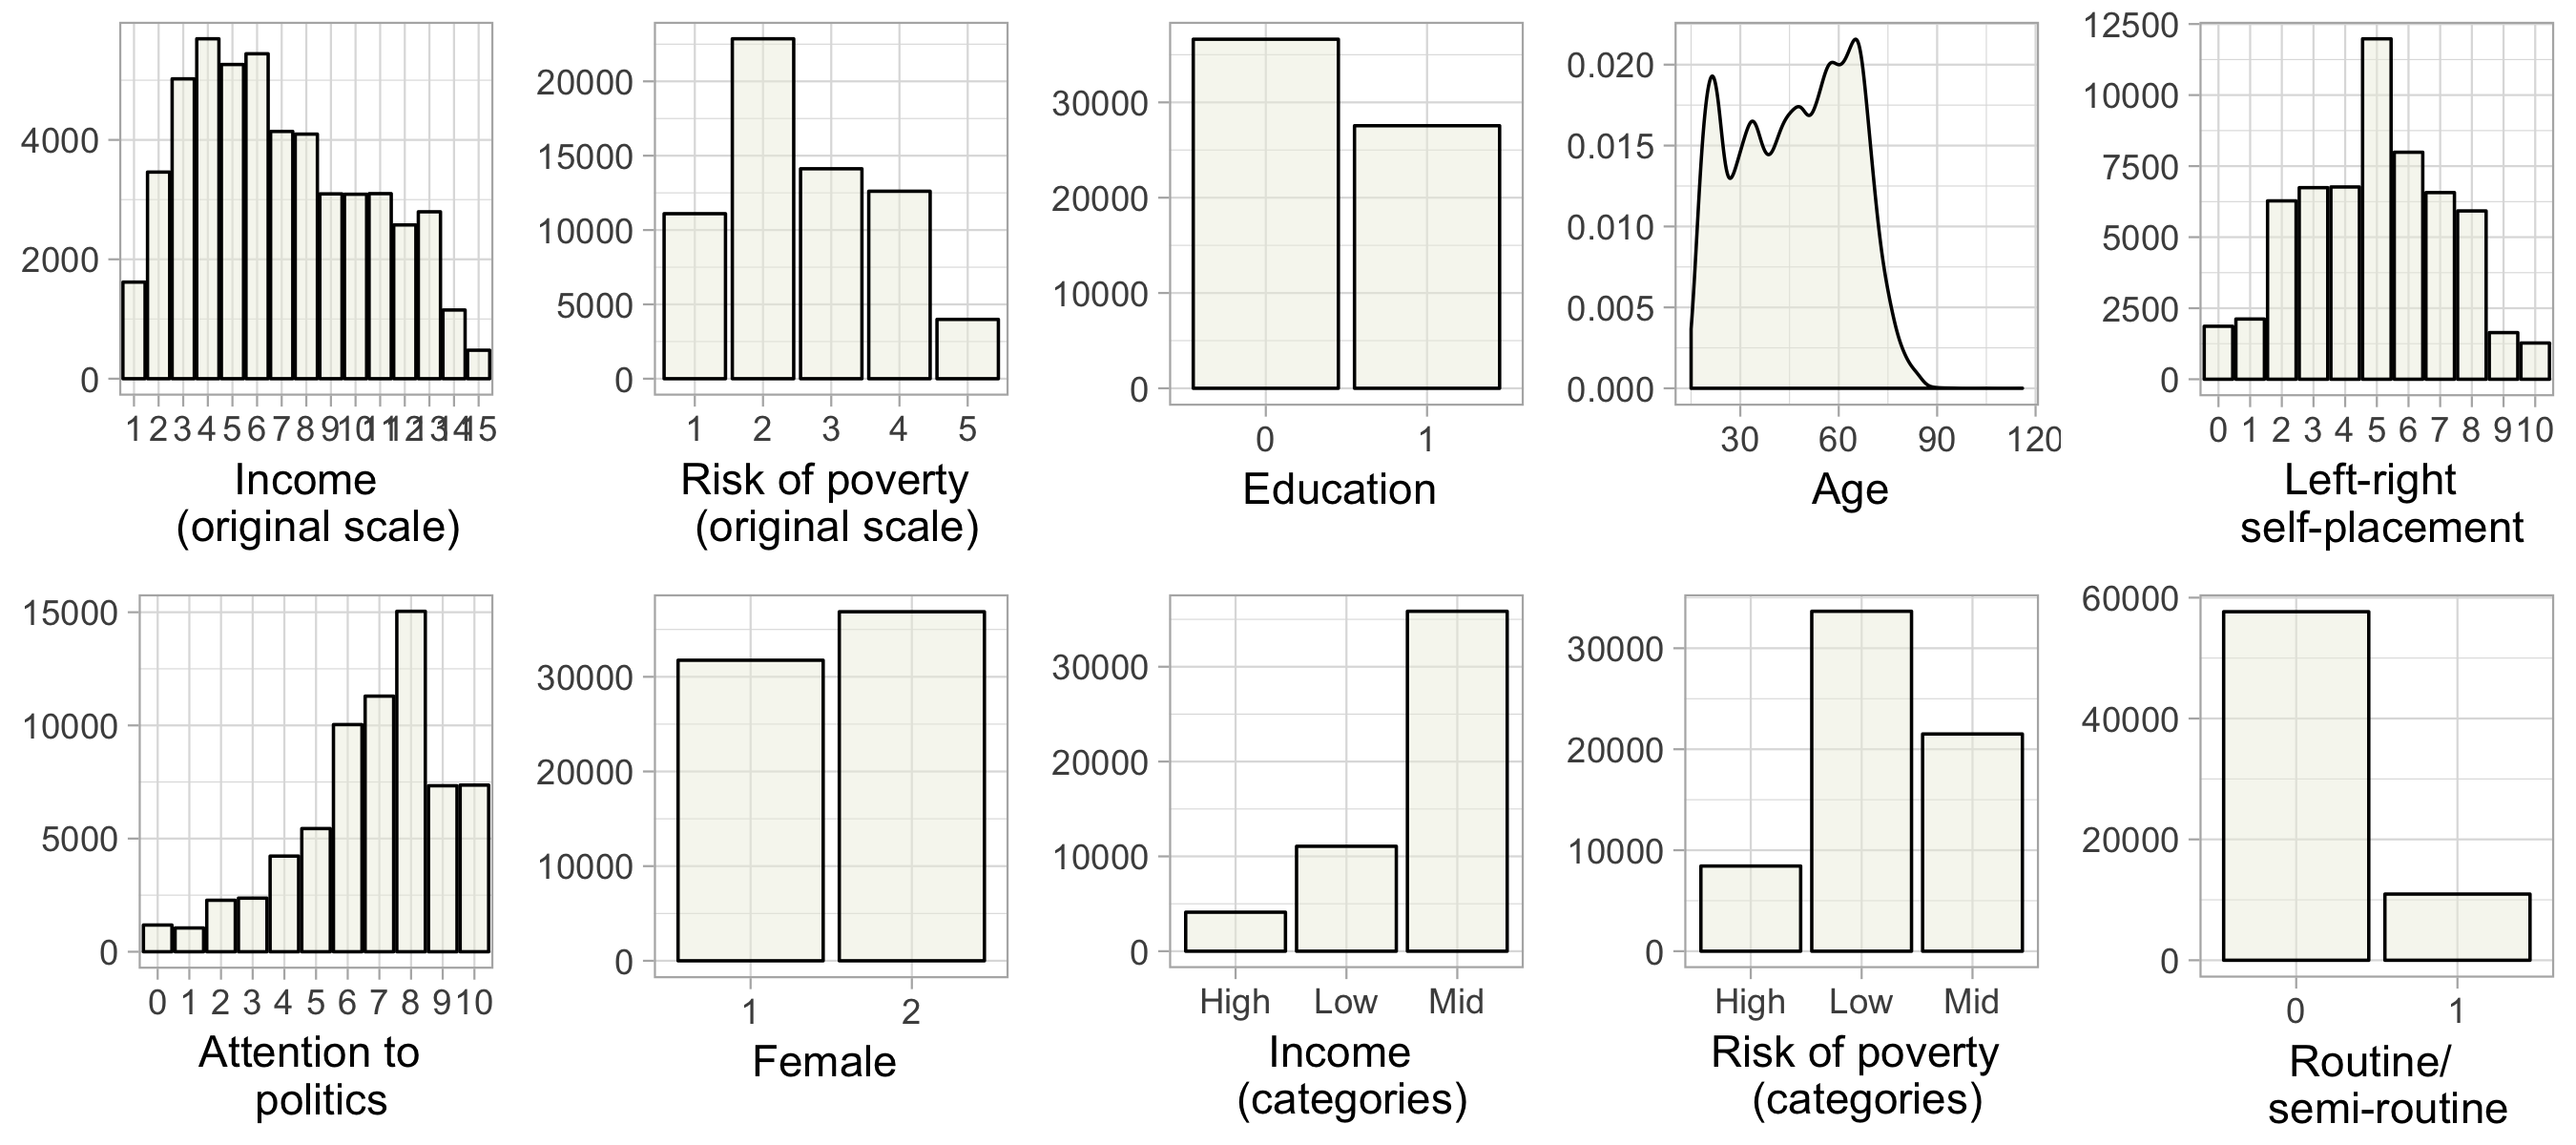
\includegraphics[scale=0.15]{ic_desc.png}
\label{fig:desc}
\end{figure}

\subsection{Descriptive statistics for dependent variables}

In the Figure~\ref{fig:desc}, I plot the descriptive statistics for the dependent variables. Once again, these are on their original scale.

\begin{figure}[H]
\centering
\caption{Distributions of dependent variables}
\vspace{10pt}
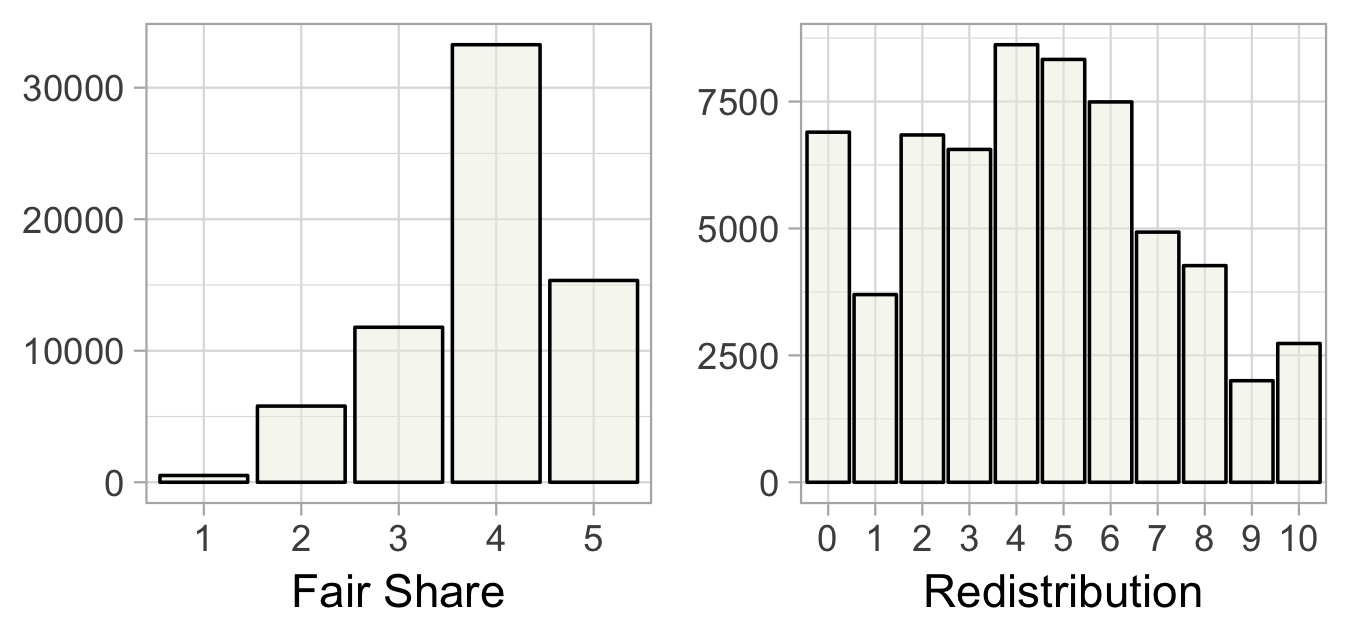
\includegraphics[scale=0.15]{ic_desc2.png}
\label{fig:desc2}
\end{figure}

\printbibliography



\end{document}